\newcommand{\DoNotLoadEpstopdf}{}
\documentclass[10pt,a4paper]{ltjsarticle}
\usepackage[margin=22mm]{geometry}
\usepackage{luatexja-fontspec}
\setmainfont{times.ttf}[Path=C:/Windows/Fonts/,BoldFont=timesbd.ttf,ItalicFont=timesi.ttf,BoldItalicFont=timesbi.ttf]
\setmainjfont{msmincho.ttc}[Path=C:/Windows/Fonts/,FontIndex=0,BoldFont=YuGothB.ttc,BoldFeatures={FontIndex=0}]
\setsansjfont{YuGothM.ttc}[Path=C:/Windows/Fonts/,FontIndex=0,BoldFont=YuGothB.ttc,BoldFeatures={FontIndex=0}]
\usepackage{amsmath,amssymb,graphicx,booktabs,multirow,xcolor,caption,subcaption}
\usepackage[hidelinks]{hyperref}
\captionsetup{font=small,labelsep=quad}
\graphicspath{{figures/}}

\title{同じカット値の CIM 解は後段の探索で同じ価値を持つか\\[2pt]
\large ——種の価値の実測，事前登録による検証，同じ総時間での選別——}
\author{}
\date{2026 年 10 月}

\begin{document}
\maketitle

\begin{abstract}
コヒーレント・イジングマシン（CIM）の出力を後段の探索の初期解（種）に使うとき，同じカット値の種は同じ価値を持つか，その差を安価に予測して選別すると役に立つかを，MAX-CUT（G-set と全列挙できる小規模問題）で調べた．種の価値は，その種から始めた焼きなまし法（SA）の最良値の期待値とした．(1) カット値と 1 反転局所探索の改善量で説明できない価値の差は，SA が種の近くを探す設定では，CIM の出力が多様な 7 問題すべてで再現した（split-half 信頼性 0.67〜0.98）．SA が種から大きく離れる設定では差は消えた．(2) 探索的に見つけた固有ベクトル指標（CIM の線形増幅で最初に成長するモードへの揃い方）を事前登録して検証し，G22 で再現した（$\rho=0.56$，95\% 区間 [0.46, 0.65]）．G1 でも同じ大きさで成り立ったが，ほかの問題では効かなかった．全列挙した小規模問題では，価値は最適解までの距離でほぼ決まり（層内 Kendall $\tau=-0.74$），エネルギー障壁の効果は弱かった．問題をまたいで同じ向きに効いた指標は，短い SA の試し打ちだけだった．(3) CIM の生成を含めた同じ総時間で比べると，カット値を超える選別は最良値をほとんど改善しなかった（最大 0.003\%）．CIM の種は，後段の予算が短い（500 掃引）とランダムな初期解より良かったが，長い（5000 掃引）と CIM の時間を SA に回したほうが良かった．(4) 後段がメメティックアルゴリズム（GA）の場合は，CIM の生成時間を含めても，CIM の初期集団がランダムな初期集団より良かった（G55・G70）．ただし，ハミング距離で多様な初期集団を選ぶと，カット値だけで選ぶより悪くなった．付随して，GA のタブー探索の同点処理の不具合を見つけて修正した．以前の「CIM の初期集団は GA に役立たない」という結論は，この不具合によるものだった．
\end{abstract}

\section{はじめに}\label{sec:intro}

コヒーレント・イジングマシン（CIM）は，光パラメトリック発振器のネットワークでイジング模型の基底状態を探す物理的な計算機である\cite{wang2013,inagaki2016,mcmahon2016}．MAX-CUT のような組合せ最適化問題を高速に近似的に解けるが，大規模な問題では出力が最適解から離れることが多く，実用上は CIM の出力を初期解として，焼きなまし法（SA）\cite{kirkpatrick1983}やメメティックアルゴリズム\cite{wu2012}などの後段の探索で磨くハイブリッドな使い方が考えられる．

このとき CIM は多数の候補を安価に生成できるので，「どの候補を後段に渡すか」が問題になる．自然な方法はカット値の高い候補を選ぶことである．しかし，同じカット値の候補でも，後段の探索で最終的に到達できる品質が同じとは限らない．候補が探索空間のどこにあるか（最適解への近さや，そこへ向かう経路の有無）によって，後段の探索の行き着く先が変わるはずである．

本論文はこの「種の価値」の差を実測し，それを安価に予測できるか，予測に基づく選別が実用上役に立つかを調べる．具体的には次の 3 つを問う．(C1) 同じカット値の CIM 解で後段の価値に差があるか．(C2) その差をカット値以外の安価な指標で予測できるか．(C3) 指標で選別すると，CIM の生成を含めた同じ総時間で到達品質が上がるか．

本論文の貢献は次のとおりである．
\begin{itemize}
  \item 同じカット値（と 1 反転局所探索の改善量）の CIM 解の間に，後段 SA での価値の再現性のある差があることを，G-set\cite{helmberg2000}で示した．差の有無は SA の設定に強く依存し，SA が種から大きく離れる設定（開始温度が高い，予算が長い）では差が消える（\ref{sec:prereg}, \ref{sec:gset} 節）．
  \item 探索的な解析で見つけた固有ベクトル指標を事前登録して新しいデータで検証し，G22 では再現することを確かめた．一方，小規模問題の検証用データと他の G-set 問題では効き方が一様でなく，局所的な指標や短い SA の試し打ちのほうが安定していた（\ref{sec:prereg}--\ref{sec:gset} 節）．
  \item 18〜24 頂点の 30 問題の全列挙により，種の価値は最適解までの距離（経路長）でほぼ決まり（層内 Kendall $\tau\approx-0.74$），エネルギー障壁はそれより弱いことを示した（\ref{sec:small} 節）．
  \item CIM の生成，指標の計算，後段の探索をすべて含めた同じ総時間での比較を行い，選別の実用上の効果を評価した（\ref{sec:selection} 節）．
  \item 付随して，メメティックアルゴリズムのタブー探索で同点の手を常に番号最小の頂点から選ぶ実装が，疎なグラフで探索を止めることを見つけ，修正と高速化を行った（\ref{sec:ga} 節）．
\end{itemize}

研究の進め方として，探索的に得た結果は，判定基準と解析を固定した事前登録の文書をリポジトリにコミットしてから新しいデータで確かめた．登録どおりの結果は，仮説を支持しないものも含めてすべて報告する．

\section{関連研究}\label{sec:related}

\paragraph{イジングマシンとハイブリッド.} CIM\cite{wang2013,inagaki2016,mcmahon2016}のほか，カオス振幅制御（CAC）\cite{leleu2019}，シミュレーテッド分岐（SB）\cite{goto2019}など，連続変数の力学で解を探す方式が提案されている．CIM の MAX-CUT 性能は SDP 緩和\cite{goemans1995}や SA と比べて評価されてきた\cite{haribara2015}．本論文はイジングマシンの出力を後段の古典的な探索に渡す使い方を対象にし，渡す候補の選び方に焦点を当てる．

\paragraph{MAX-CUT の発見的解法.} G-set\cite{helmberg2000}に対しては，ブレイクアウト局所探索（BLS）\cite{benlic2013}，メメティックアルゴリズム\cite{wu2012}，複数の探索演算子を使う MOH\cite{ma2017}などが高い性能を示している．Dunning ら\cite{dunning2018}は多数の解法を体系的に比較した．本論文の目的は最良値の更新ではなく，CIM と後段の探索をつなぐ部分の設計である．

\paragraph{初期解の選び方と地形.} 局所最適解の網（local optima network）\cite{ochoa2008}は，探索空間の地形を局所最適解とその間の遷移で表し，探索の難しさを説明する．本論文の障壁・経路長はこれと同じ問題意識を，個々の初期解について厳密に測ったものである．強化学習で解を改善する方法\cite{barrett2020}も，初期状態からどこへ到達できるかを学習している．計算予算の配分の観点では，短い試行で候補を絞る successive halving\cite{karnin2013,jamieson2016}が，本論文の「試し打ち」に相当する強い比較相手である．

\paragraph{スペクトル的な手法.} MAX-CUT と隣接行列の最小固有値・固有ベクトルの関係は，スペクトル的な丸めとして知られている\cite{trevisan2012}．CIM の増幅初期は線形写像で近似でき，結合行列の最大固有値の固有モードが先に成長するので，CIM の出力がそのモードに偏ることが考えられる．本論文の固有ベクトル指標は，この偏りを候補ごとに測るものである．

\section{問題設定と方法}\label{sec:method}

\subsection{種の価値}

重み $w_{ij}$ を持つグラフ $G=(V,E)$，$|V|=n$ の MAX-CUT を考える．解はスピン $s\in\{-1,+1\}^n$ で表し，カット値を $c(s)=\sum_{(i,j)\in E} w_{ij}[s_i\neq s_j]$ とする．全反転 $s\mapsto -s$ は同じ解とみなす．

CIM の 1 回の実行が出力する解を\textbf{候補}（種）と呼ぶ．候補 $s$ を初期解として後段の探索 $\mathcal{A}$（本論文では主に SA）を予算 $B$ で 1 回実行したときの最良カット値を確率変数 $Y_{\mathcal{A},B}(s)$ とし，その期待値
\begin{equation}
  V_{\mathcal{A},B}(s) = \mathbb{E}\left[Y_{\mathcal{A},B}(s)\right]
\end{equation}
を候補の\textbf{価値}と呼ぶ．期待値は後段の探索の乱数についてとる．本論文の問いは次の 3 つである．

\begin{description}
  \item[C1（現象）] 同じカット値の候補でも $V$ が異なるか．
  \item[C2（説明）] その差を，カット値以外の安価な指標で予測できるか．
  \item[C3（実用）] 指標で候補を選ぶと，CIM の生成を含めた同じ総時間で到達品質が上がるか．
\end{description}

\subsection{CIM と後段の探索}

\paragraph{CIM.} 位相感応増幅器と測定フィードバックを持つファイバーループ型 CIM の進行波モデル\cite{inoue2022}を用いる（CIM 全般は\cite{wang2013,inagaki2016,mcmahon2016}）．ポンプ強度をラウンドごとに一定量（\texttt{dP\_per\_round}）ずつ上げ，各ラウンドで結合 $J=cA$（$A$ は重み付き隣接行列，$c<0$）を通したフィードバックと真空雑音を加える．各実行で，途中で最もカット値の高かった符号を出力とする．パラメータは，G22 について以前の研究で調整した物理定数を用い，問題ごとに結合の強さ $c$ だけを CIM 単体の平均カット値が最大になるように選んだ（後段のラベルは見ていない）．

\paragraph{SA.} 後段の探索は，1 反転提案ごとに温度を指数的に下げる SA\cite{kirkpatrick1983}である．初期解 $s$ から出発し，途中の最良状態（初期解を含む）を返す．予算は反転提案の総数で表し，頂点数で割った値を\textbf{掃引}と呼ぶ．開始温度 $T_0$ は，warm start 向けの $0.5$，冷却 SA の既定値 $2.0$，以前の研究で G22 向けに調整した $4.21$ を用いた．終了温度は $0.001$（調整済みの設定のみ $0.052$）である．

\paragraph{ラベル.} 候補ごとに SA を $R$ 回（互いに異なる乱数）実行し，最良カット値の平均 $\bar{y}(s)$ を $V(s)$ の推定値（ラベル）とする．小規模問題では，SA が最適値に到達した割合をラベルとした．

\subsection{同じカット値の候補の比較}

CIM の出力は 1 反転の局所最適解とは限らず，貪欲な 1 反転局所探索（LS）でただちに改善できることが多い．この「すぐ取れる改善」で説明できる差は自明なので，C1・C2 では，ラベルを初期カット値 $c(s)$ と LS 後のカット値 $c_{\mathrm{LS}}(s)$ で回帰した残差
\begin{equation}
  r(s) = \bar{y}(s) - \left(\beta_0 + \beta_1 c(s) + \beta_2 c_{\mathrm{LS}}(s)\right)
\end{equation}
を対象にする（係数は問題・条件ごとの最小二乗推定）．

\paragraph{C1 の判定.} $R$ 回の SA を偶数回目と奇数回目の 2 群に分け，各群の平均で残差を作り，その相関に Spearman--Brown 補正をかけた値（残差の split-half 信頼性）を求める．SA の乱数は 2 群で独立なので，この値は「カット値と LS で説明できない，候補に固有の価値」がどれだけ再現するかを表す．0.3 以上かつ候補ブートストラップの 95\% 区間の下限が 0 を超えれば，差があると判定した．

\paragraph{C2 の判定.} 指標と残差 $r$ の Spearman 順位相関 $\rho$ と，候補ブートストラップ（各標本で回帰し直す）の 95\% 区間を求める．小規模問題では，候補を（問題，初期カット値）の層に分け，層内の Kendall $\tau_b$ を候補数で重み付け平均した値と，層内で平均を引いた値どうしの相関の 2 乗（偏 $R^2$）を用いた．区間は問題を単位にしたブートストラップで求めた．

\subsection{指標}

\paragraph{固有ベクトル指標.} CIM の増幅は，しきい値の近くでは線形写像 $c_{k+1}\approx g(\sqrt{\eta}I+J)c_k+\xi$ で近似でき，$J$ の最大固有値の固有ベクトルが最初に成長する．$J=cA$（$c<0$）なので，これは $A$ の最小固有値側の固有ベクトルにあたる．$A$ の最小固有値側の 2 本を $u_1,u_2$（固有値の昇順）とし，
\begin{equation}
  a_j(s) = \frac{\left|\langle s, \operatorname{sign}(u_j)\rangle\right|}{n},\qquad E(s) = a_1(s) - a_2(s)
\end{equation}
を定義する．$a_j$ は候補が $u_j$ の符号パターンにどれだけ揃っているかを表す．MAX-CUT と $A$ の最小固有値の関係は Trevisan\cite{trevisan2012}がスペクトル的な丸めとして論じている．固有ベクトルは問題ごとに 1 回だけ計算すればよく，各候補では内積だけで評価できる．

\paragraph{局所的な指標.} 各頂点を反転したときのカットの増分 $g_i$ から，$g_i=0$ の頂点数（\texttt{n\_zero\_gain}），$-2\le g_i\le 0$ の頂点数（\texttt{n\_gain\_minus2\_to\_0}），$g_i=0$ の頂点がつくる連結成分の最大サイズなどを求める．LS 後の解についても同じ量を求める（接頭辞 \texttt{ls\_}）．いずれも辺数に比例する時間で計算できる．

\paragraph{試し打ち.} 候補に短い SA（大規模問題では 50 掃引を 2 回，小規模問題では 1 掃引を 8 回）をかけた結果の平均を指標とする．計算費用は大きいが，候補の後段での振る舞いを直接見る強い比較相手である．

\subsection{厳密量（小規模問題）}

18〜24 頂点の問題では，全反転を同一視した $2^{n-1}$ 状態を全列挙し，次の量を厳密に求めた．
\begin{description}
  \item[障壁] $B(s)=c(s)-\ell^*(s)$．$\ell^*(s)$ は，カット値が $\ell$ 以上の状態だけを 1 反転でたどって $s$ から最適解に行ける最大の $\ell$．$B=0$ ならカット値を下げずに最適解に行ける．状態をカット値の高い順に加えながら素集合森で連結成分を管理して求めた．
  \item[経路長] カット値が $\ell^*(s)$ 以上の状態だけを通る，$s$ から最適解までの最短の反転回数．最適解からの幅優先探索で求めた．
  \item[最適解までの距離] 最も近い最適解とのハミング距離．
\end{description}
全列挙のカット値と，障壁・経路長は，8〜9 頂点の問題で素朴な全探索の結果と一致することを確かめた．

\section{事前登録した確認実験}\label{sec:prereg}

\subsection{経緯と登録の内容}

探索段階（G22，CIM 600 ラウンド，seed 0〜255，SA 開始温度 2.0）で，予算 $10^7$ 反転提案（5000 掃引）の SA 後の価値の残差 $r$ と固有ベクトル指標 $E$ の間に順位相関 $\rho=0.57$ が見つかった．指標の定義と使う固有ベクトルの本数はデータを見てから選んだので，定義，解析，判定基準（$\rho$ の 95\% 区間の下限 $>0$）を文書に固定してリポジトリにコミットした後，新しい CIM seed（256〜511）で確かめた．実行は表\ref{tab:prereg}の R1〜R5 の 5 つで，主検定は探索段階と同じ手順の R1 である．候補は $K=256$，SA は各候補 $R=16$ 回で，予算は 50・500・5000 掃引の 3 段階とし，5000 掃引を主予算とした．

\begin{table}[t]
\centering
\caption{事前登録した確認実験の結果（主予算 5000 掃引）．C1 は残差の split-half 信頼性．距離は SA の出力と種のハミング距離の平均（全反転を同一視，頂点数で正規化）．}\label{tab:prereg}
\small
\begin{tabular}{llcccc}
\toprule
実行 & 条件 & $\rho(E, r)$ [95\% 区間] & 判定 & C1 & 距離 \\
\midrule
R1 & G22，600 ラウンド，$T_0=2.0$（主検定） & $0.56$ [$0.46$, $0.65$] & 再現 & $0.89$ & $0.26$ \\
R2 & G22，600 ラウンド，$T_0=4.21$（調整済み） & $-0.02$ [$-0.14$, $0.10$] & 再現せず & $-0.01$ & --- \\
R3 & G22，2400 ラウンド，$T_0=2.0$ & $0.54$ [$0.44$, $0.62$] & 再現 & $0.89$ & $0.26$ \\
R4 & G55，2400 ラウンド，$T_0=2.0$ & $-0.03$ [$-0.15$, $0.10$] & 再現せず & $0.07$ & $0.43$ \\
R5 & G70，2400 ラウンド，$T_0=2.0$ & $0.06$ [$-0.06$, $0.18$] & 再現せず & $0.20$ & $0.44$ \\
\bottomrule
\end{tabular}
\end{table}

\begin{figure}[t]
\centering
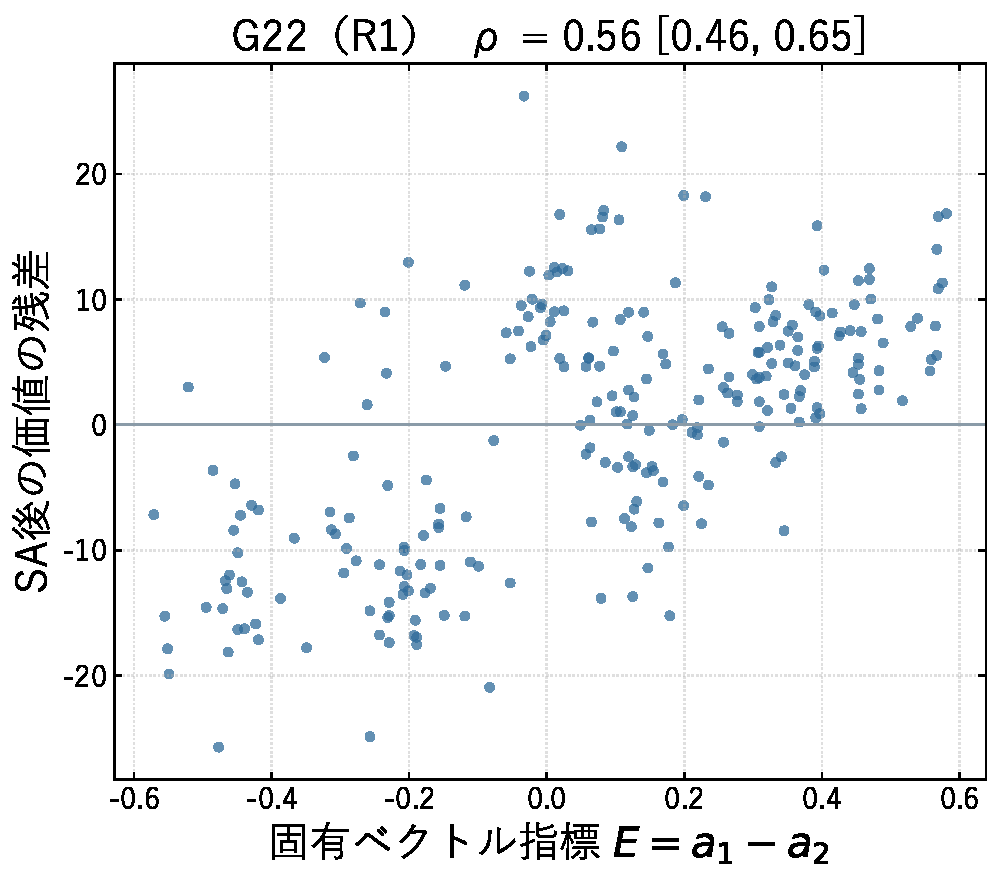
\includegraphics[width=0.42\linewidth]{fig_prereg_scatter.pdf}
\caption{主検定 R1（G22）の候補 256 個．横軸は固有ベクトル指標 $E$，縦軸は SA（5000 掃引）後の価値を初期カット値と LS 後のカット値で回帰した残差．$E$ はいくつかの値の近くに集まり，候補が固有ベクトルの「系統」に分かれることを示す．}\label{fig:prereg_scatter}
\end{figure}

\begin{figure}[t]
\centering
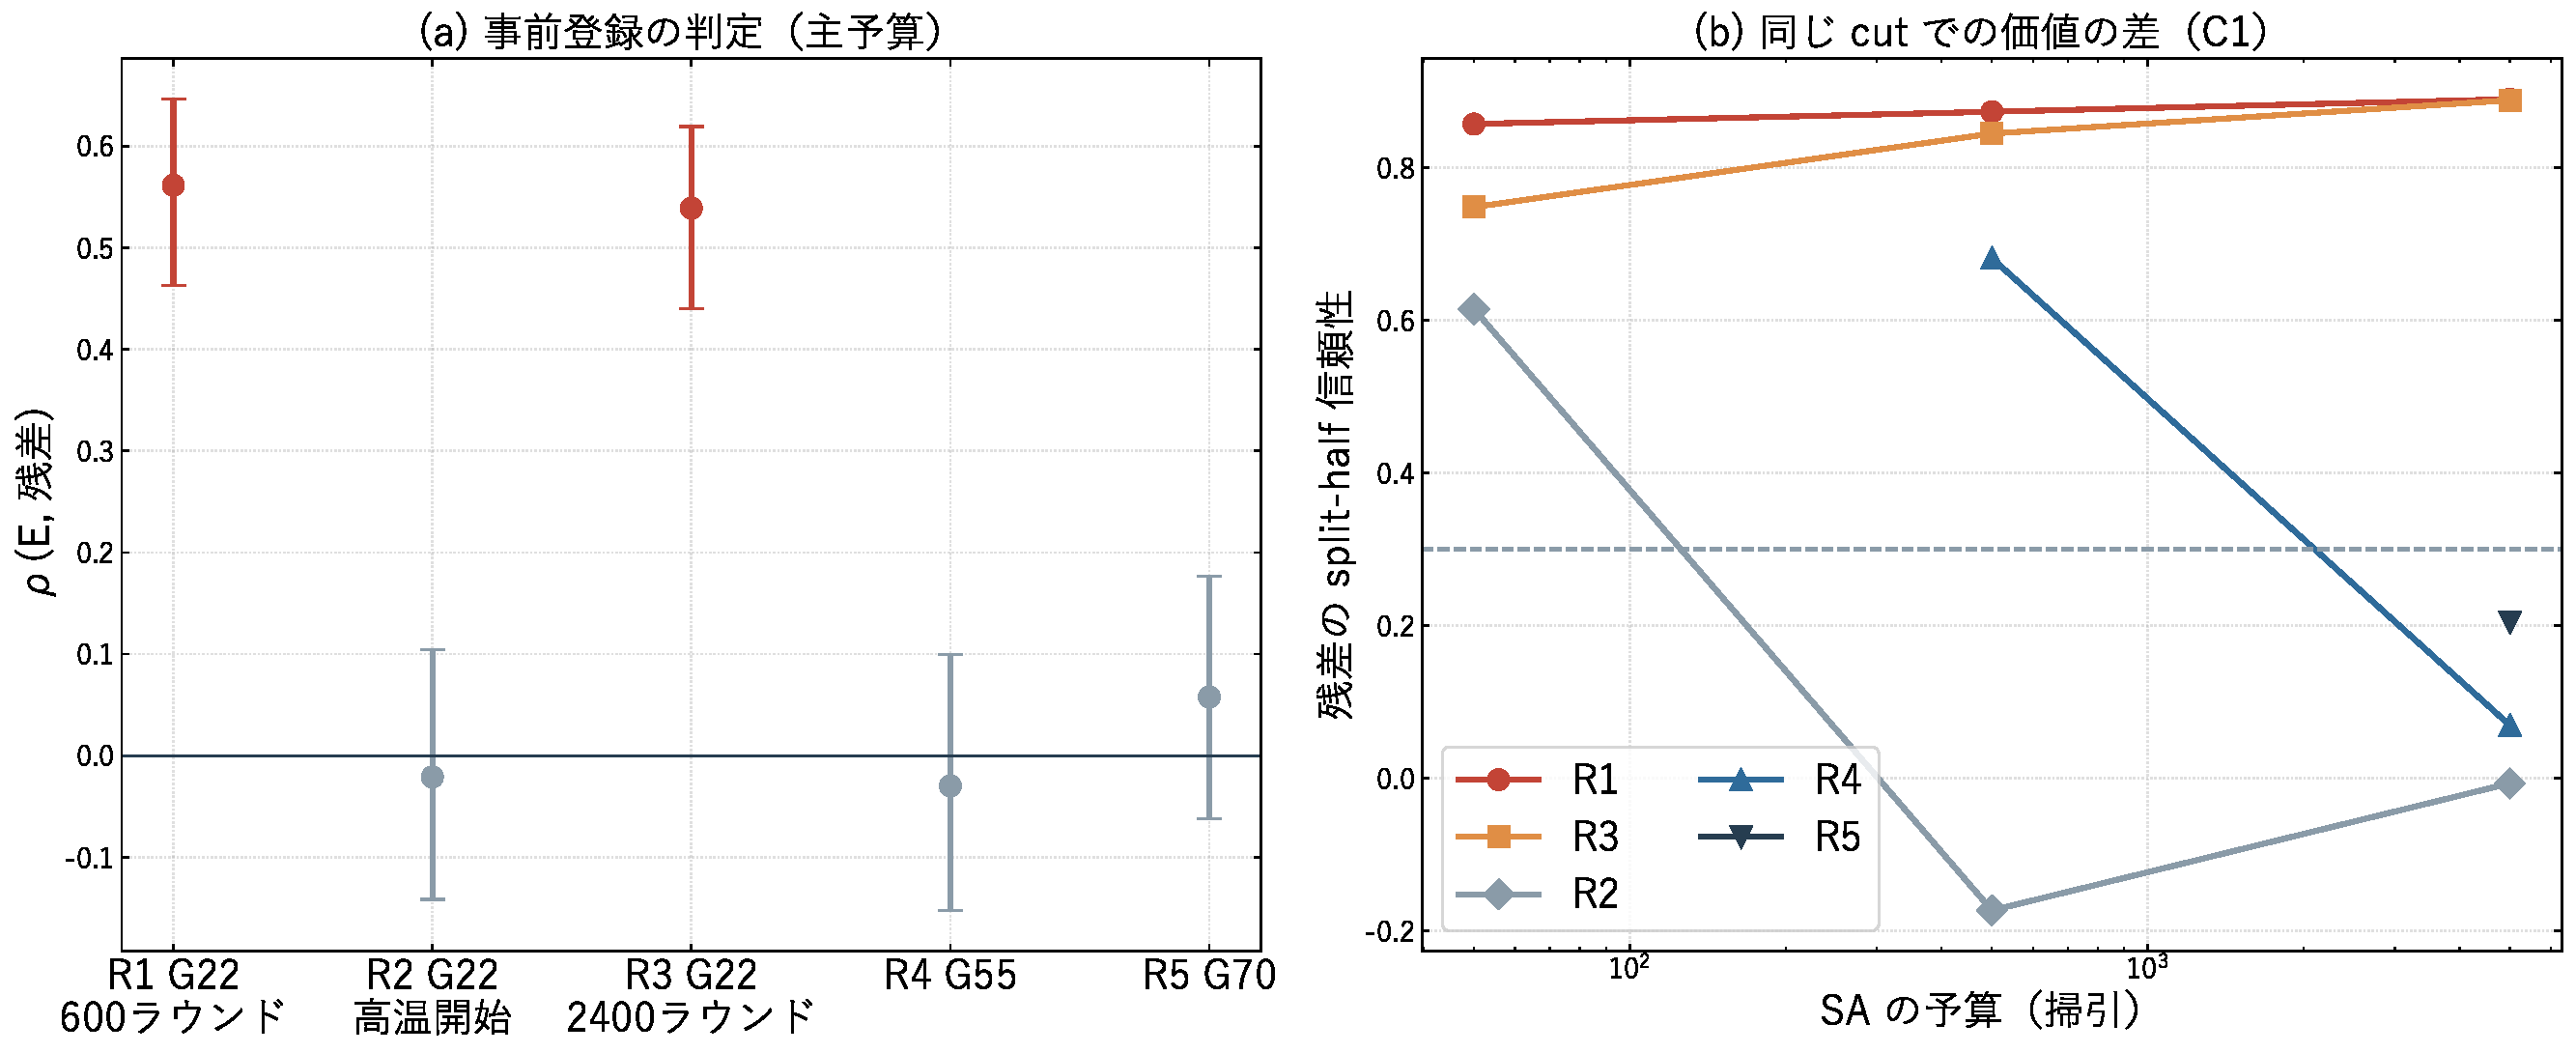
\includegraphics[width=\linewidth]{fig_prereg_summary.pdf}
\caption{(a) 各実行の主予算での $\rho(E, r)$ と 95\% 区間（赤は再現）．(b) 残差の split-half 信頼性（C1）と SA の予算．点線は判定基準 0.3．SA が種を一度も超えずラベルが初期カット値と一致した条件（R4 の 50 掃引，R5 の 50・500 掃引）は判定不能として除いた．}\label{fig:prereg_summary}
\end{figure}

\subsection{結果}

主検定 R1 は再現した（$\rho=0.56$，95\% 区間 [$0.46$, $0.65$]，図\ref{fig:prereg_scatter}）．$E$ は残差の分散の 39\% を説明し，これは SA の乱数で再現できる部分（信頼性 0.89）の 44\% にあたる．CIM を収束まで回した R3 でも同じ大きさで再現した．したがって G22 では，CIM 出力がどちらの固有ベクトルの符号パターンに揃っているかが，カット値と局所探索の改善量では説明できない後段の価値を予測する．

一方，残りの 3 つの実行では再現しなかった．注目すべきは，これらの条件ではそもそも予測すべき差がほとんどなかったことである（図\ref{fig:prereg_summary}(b)）．調整済みの高い開始温度（R2）や，G55・G70 の長い予算（R4・R5）では，SA の出力は種から頂点の 43〜44\% も離れ，残差の信頼性は 0.07〜0.20 に下がった．SA が種をほとんど「忘れる」設定では，同じカット値の候補の価値は等しくなる．G55 の 500 掃引では差が残った（信頼性 0.68）が，$E$ はその差を予測しなかった（$\rho=-0.02$）．

\paragraph{登録後の変更.} warm SA は途中の最良状態（初期解を含む）を返すので，開始温度が高く予算が短いと，SA が一度も種を超えずにラベルが初期カット値と一致する（R4 の 50 掃引，R5 の 50・500 掃引）．このとき残差は恒等的に 0 になり，判定量が定義できない．登録時にはこの場合を想定していなかったので，解析を直してこの場合を判定不能とした．主予算の判定には影響しない．

\paragraph{二峰性について.} 探索段階では，G22 の SA 後の価値が約 13315 と 13345 の 2 群に分かれることを観察していた．同じ判定（GMM の 1 成分と 2 成分の BIC 差 $>10$，Ashman の $D>2$）を当てはめると，ラベルは探索段階・R1・R3 のいずれでも二峰だった．しかし，その由来は一貫しなかった．探索段階では初期カット値が二峰で残差は二峰でなく，R1 では初期カット値は二峰でなく残差が二峰（BIC 差 18.9，$D=3.1$），R3 ではどちらも二峰でなかった．ラベルの二峰性は再現するが，それが初期カット値の分布によるのか，カット値で説明できない部分によるのかは，本論文のデータでは決められない．

\section{小規模問題での厳密な解析}\label{sec:small}

\subsection{設定}

18〜24 頂点の問題を 30 個作った．種類は，ランダム 3 正則グラフ（重み 1），平均次数 4 の Erdős--Rényi グラフに重み $\pm1$ をつけたもの，$4\times5$・$4\times6$ の格子に確率 0.6 で対角辺を加えた三角格子（重み 1）を各 10 個である．番号の偶数・奇数で開発用と検証用に 15 個ずつ分け，指標と仮説は開発用だけを見て決め，その文書をコミットしてから検証用を解析した．

小規模問題では，CIM を 1500 ラウンド回すとほぼ必ず最適解を出す（最適率 0.95 以上）．大規模問題では CIM の出力は最適解の手前（G-set で最適値との差 0.3〜3\%）にあるので，同じ状況を作るため，増幅の途中の 512 ラウンドで止めた CIM を 1024 回実行し，異なる非最適解を候補とした．1 問題（$\pm1$ 重みの 1 つ）は CIM が常に最適解を出したので除き，29 問題で計 8647 個の候補を得た．各候補に SA（開始温度 0.5，終了温度 0.01）を 256 回かけ，3・10・30 掃引で最適値に到達した割合をラベルとした．候補が 5 個以上ある（問題，初期カット値）の層で比べた．

\subsection{結果}

図\ref{fig:small}に，10 掃引のラベルに対する層内の Kendall $\tau$ を示す．

\begin{figure}[t]
\centering
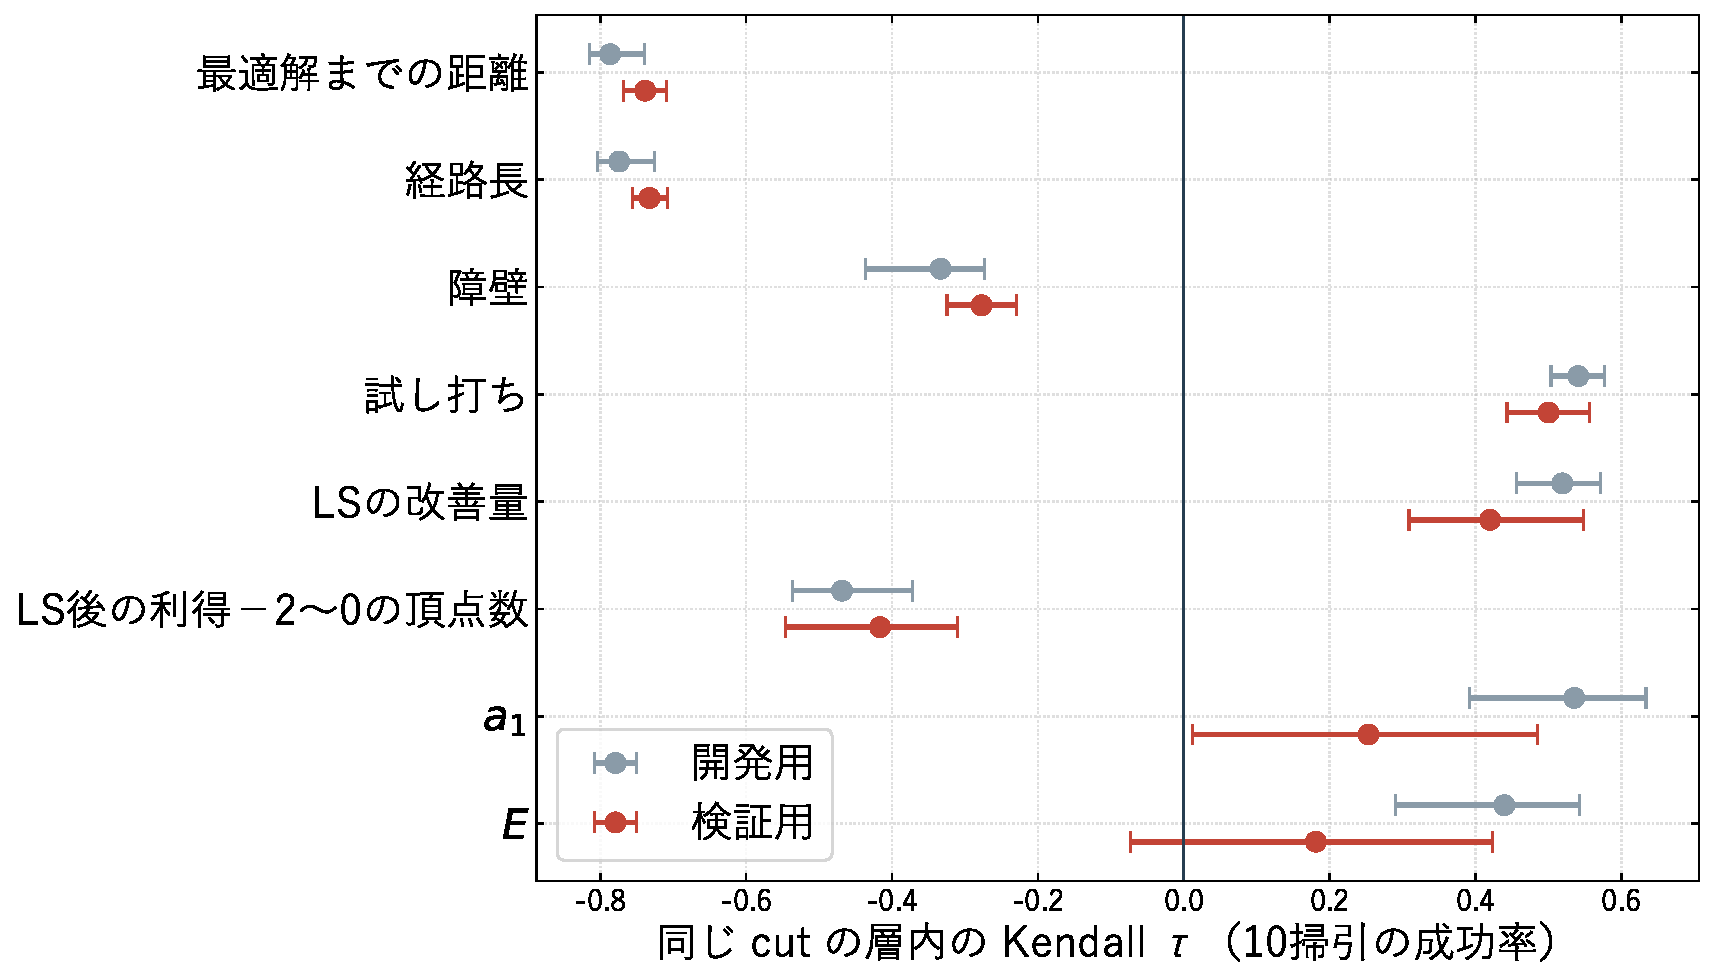
\includegraphics[width=0.72\linewidth]{fig_small_tau.pdf}
\caption{小規模問題で，同じ初期カット値の候補の中での，指標と SA の最適到達率（10 掃引）の Kendall $\tau$．灰色は開発用 14 問題，赤は検証用 15 問題．区間は問題を単位にしたブートストラップの 95\% 区間．}\label{fig:small}
\end{figure}

\paragraph{種の価値はほぼ最適解までの距離で決まる.} 厳密量のうち，最適解までのハミング距離（検証用 $\tau=-0.74$，偏 $R^2=0.65$）と経路長（$-0.73$，$0.60$）が最も強く，両者はほぼ同じ量だった（互いの $\tau=0.97$）．障壁は弱かった（$-0.28$，$0.26$）．多くの候補はカット値を下げずに最適解へ行け（障壁 $>0$ の候補は問題ごとに 0〜29\%），後段の SA にとっての難しさは「越えるべき山の高さ」より「進むべき距離」で決まっていた．

\paragraph{局所的な指標と試し打ちは安定して効く.} 試し打ち（1 掃引の SA を 8 回，$\tau=0.50$），LS の改善量（$0.42$），LS 後に利得が $-2$〜$0$ の頂点数（$-0.42$）は，開発用と検証用で同程度に効いた．試し打ちと LS の改善量は，3 種類の問題のいずれでも区間が 0 を含まなかった．

\paragraph{固有ベクトル指標は問題によって効き方が違う.} 開発用では $a_1$ が強かった（$\tau=0.54$）が，検証用では $0.25$（[$0.01$, $0.49$]）に下がった．事前登録の $E$ は検証用で確認できなかった（$0.18$，[$-0.07$, $0.42$]）．種類別に見ると，3 正則グラフと三角格子では開発用で $\tau=0.49$〜$0.61$ と強いが，$\pm1$ 重みのグラフではほぼ効かない（開発用 $0.20$，検証用 $0.02$）．また，検証用でも問題ごとのばらつきが大きく，区間が広い．一方，$a_1$ は最適解までの距離と対応していた（検証用 $\tau=-0.30$，[$-0.56$, $-0.04$]）．$u_1$ の符号パターンに近い候補は最適解にも近い傾向があり，固有ベクトル指標が効くときの仕組みは「最適解への近さの粗い代理」と解釈できる．

\paragraph{予算への依存.} 3 掃引では試し打ちと局所的な指標の偏 $R^2$ が大きく，30 掃引では最適解までの距離の偏 $R^2$ が大きくなった（開発用で 3・10・30 掃引の順に 0.59，0.70，0.74）．短い予算では「すぐ取れる改善」が，長い予算では大域的な位置が効くという傾向は，G22 で $E$ が長い予算でだけ効いたこと（表\ref{tab:prereg}）と整合する．

\section{G-set の 9 問題での検証}\label{sec:gset}

\subsection{設定}

事前登録の結果（\ref{sec:prereg} 節）と小規模問題の結果（\ref{sec:small} 節）を受けて，判定基準を実行前に固定した計画をコミットしてから，G-set の 9 問題で C1・C2 を調べた．問題は，ランダムグラフ G1（800 頂点），G22，G23（2000），G55（5000），G70（10000），平面グラフ G14，G15（800），G39（2000），トーラス G32（2000）である．重みは G32 と G39 が $\pm1$，ほかは 1 である．計画には G77（トーラス，14000 頂点）も含めていたが，計算時間の都合で，結果を見る前に除いた．

CIM は 2400 ラウンド（全問題で収束を確認）とし，事前登録の実行と重ならない seed で各問題 $K=512$ 個の候補を作った．SA は開始温度 $T_0=0.5$ と $2.0$，予算 50・500・5000 掃引で，各候補に $R=16$ 回かけた．試し打ちは 50 掃引の SA を 2 回とした．問題 × 温度 × 予算の 54 条件で，C1（残差の split-half 信頼性）と指標ごとの $\rho$ を求めた．

固定した判定は次の 4 つである．
\begin{description}
  \item[H3a] CIM の出力が多様な問題（異なる状態が候補の半分以上）では，$T_0=0.5$ のいずれかの予算で C1 が成り立つ．
  \item[H3b] $T_0=2.0$・5000 掃引で C1 が成り立つ問題では，$\rho(E,r)$ の区間の下限が 0 を超える（主検定 R1 の一般化）．
  \item[H3c] C1 が成り立つ条件では，試し打ちの $\rho$ の区間の下限が 0 を超える．
  \item[H3d] C1 が成り立つ条件では，LS 後に利得が $-2$〜$0$ の頂点数の $\rho$ の区間の上限が 0 を下回る（小規模問題での向き）．
\end{description}

\paragraph{解析後の変更.} 事前登録と同じく，SA が種を超えずラベルが初期カット値と一致する条件は判定不能とする計画だった．しかし判定に使っていた「残差の幅 $<10^{-9}$」は，カット値が $10^4$ 程度の問題では最小二乗の丸め誤差で通り抜け，G55（$T_0=2.0$・50 掃引）で見かけの C1 $=1.00$ が出た．また G70（$T_0=2.0$・50・500 掃引）では，512 候補のうち 1 候補だけが種を超え，相関がその 1 候補で決まっていた．そこで「SA が種を一度でも超えた候補が 5\% 未満なら判定不能」に改め，この 3 条件を判定不能とした．ほかの 51 条件の値は変わらない．

\subsection{結果}

図\ref{fig:gset}に全条件の結果を示す．C1 が成り立ったのは 54 条件中 33 条件だった．

\begin{figure}[t]
\centering
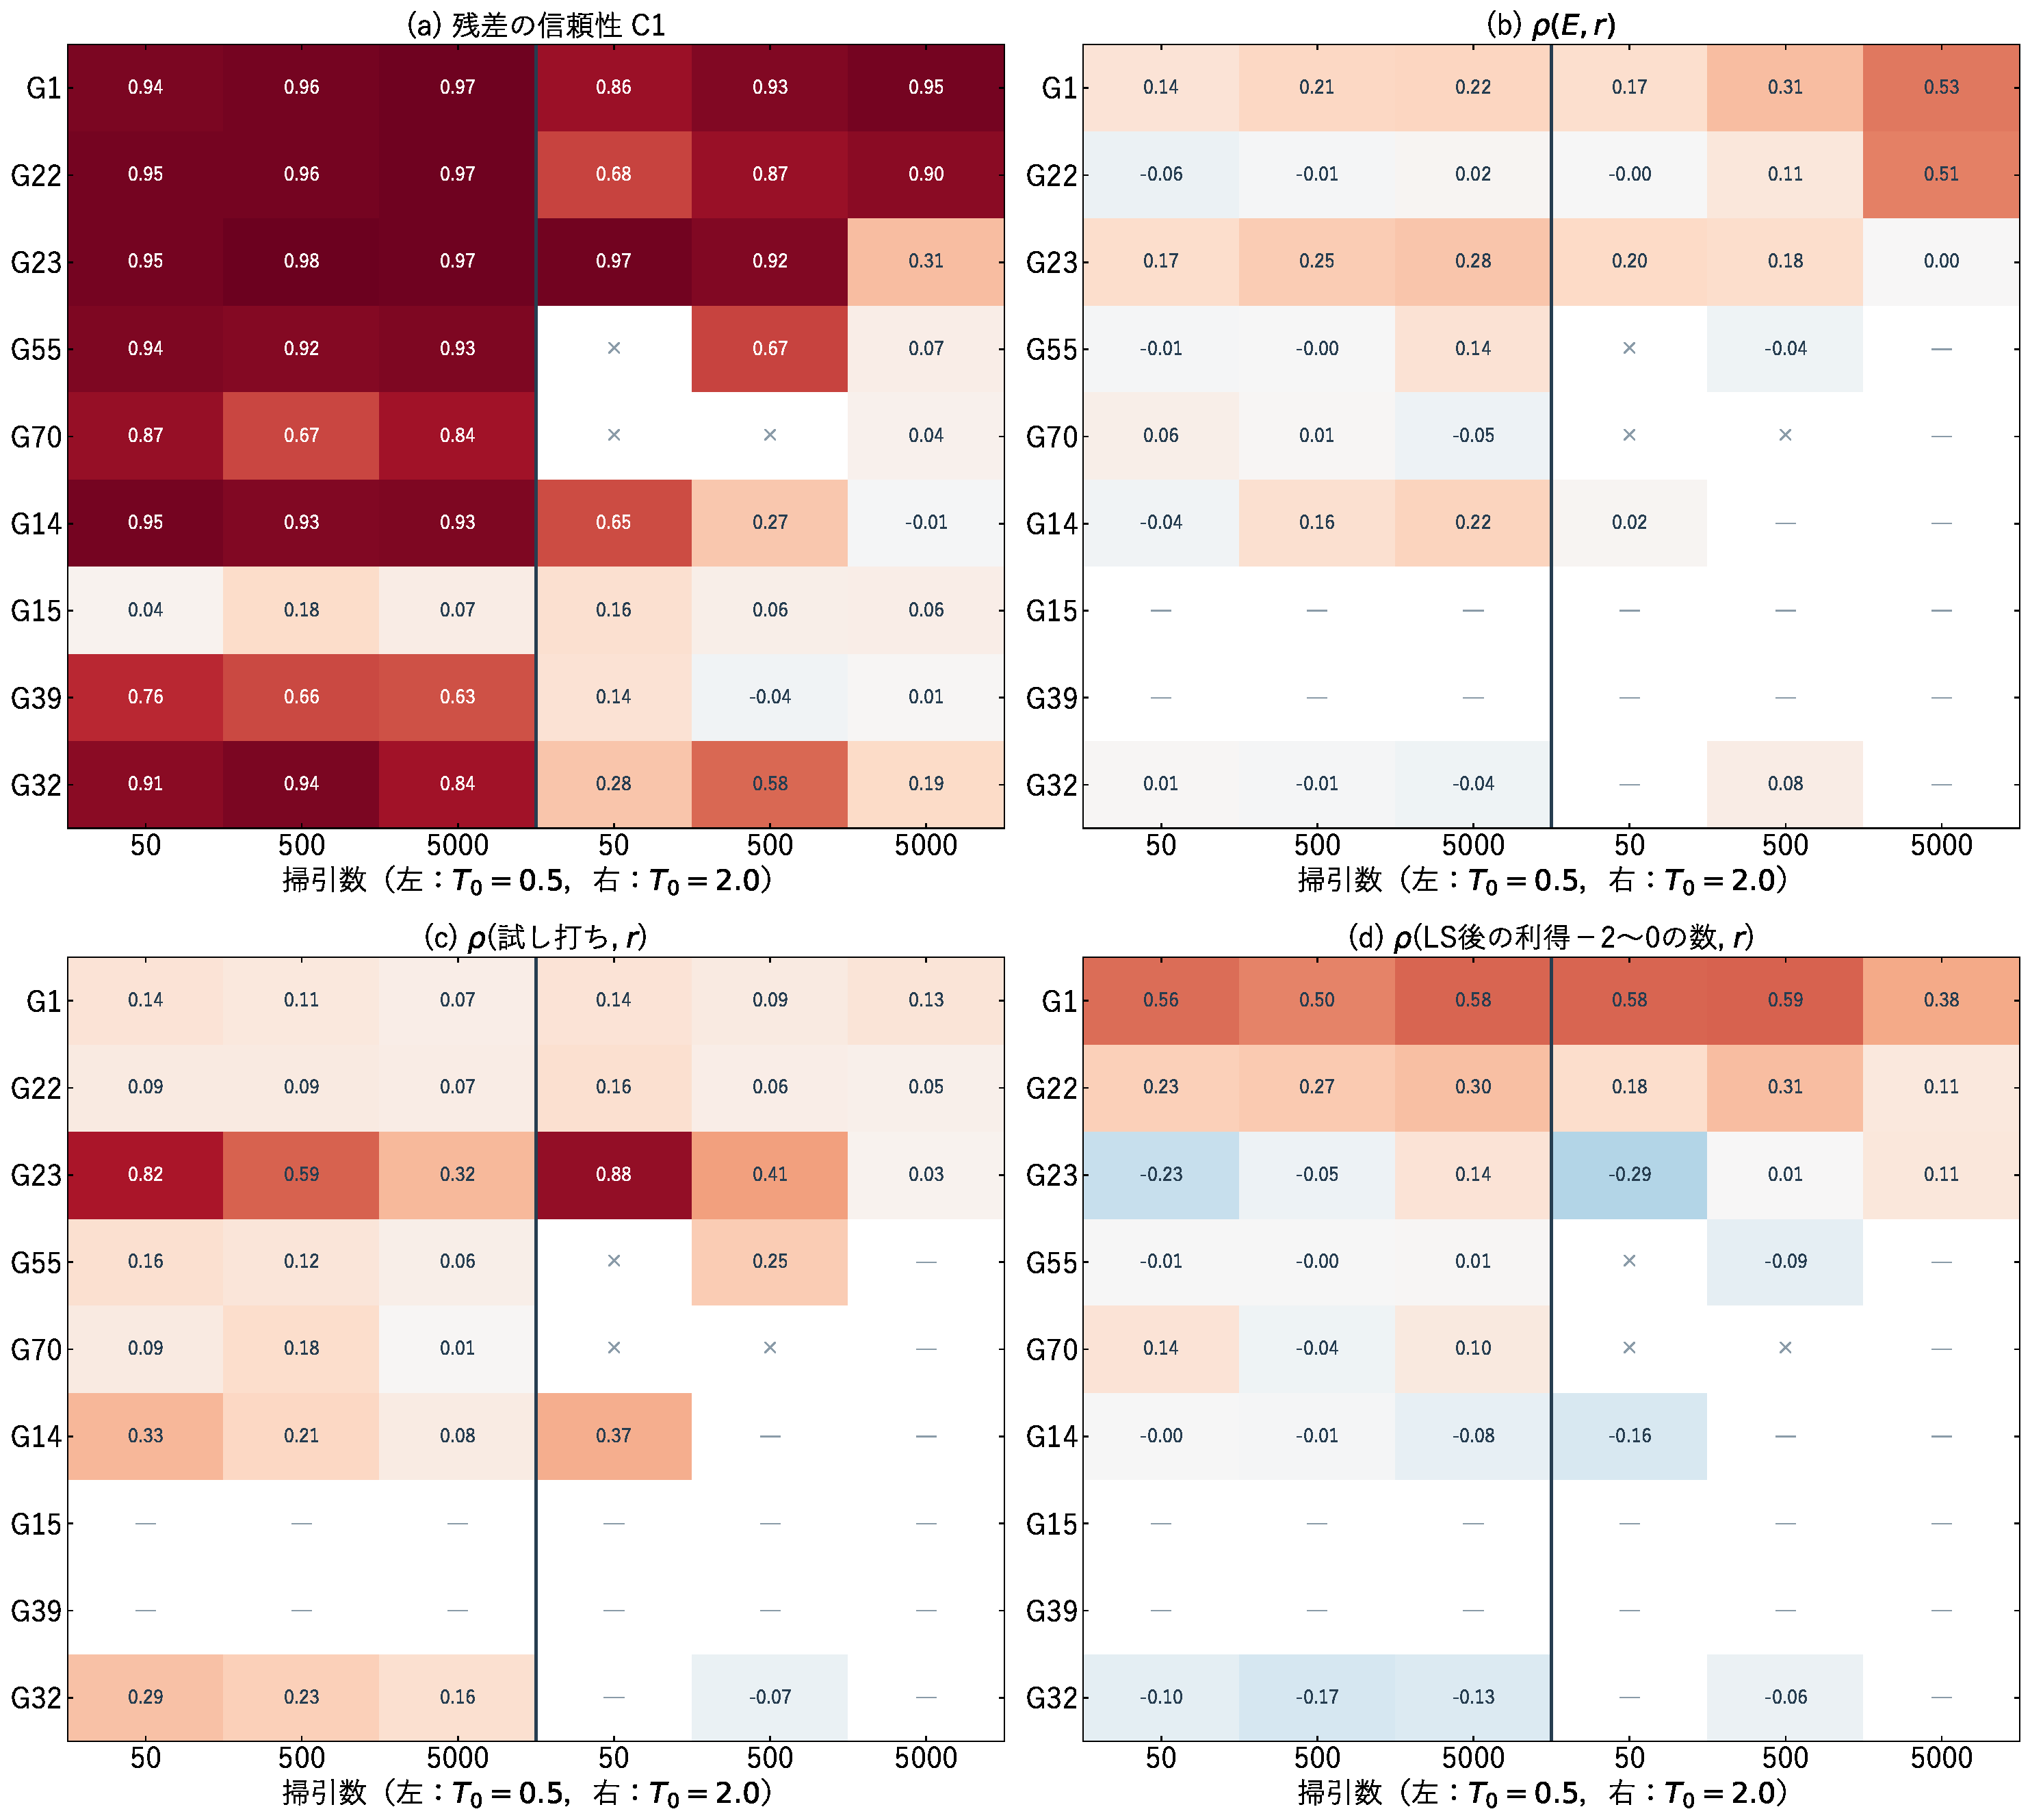
\includegraphics[width=\linewidth]{fig_gset.pdf}
\caption{G-set の 9 問題の結果．各マスは問題 × 開始温度 × 予算．(a) 残差の split-half 信頼性．(b)〜(d) 指標と残差の Spearman $\rho$（C1 が成り立った条件だけ色をつけた）．「×」は判定不能（SA が種をほとんど超えない），「—」は C1 が成り立たない条件．}\label{fig:gset}
\end{figure}

\paragraph{C1 は CIM の出力が多様なら成り立つ（H3a 成立）.} 出力が多様な 7 問題（異なる状態 303〜512 個）のすべてで，$T_0=0.5$ の 3 つの予算すべてで C1 が成り立った（信頼性 0.67〜0.98）．$T_0=0.5$ の SA は種の近くを探すので，カット値と LS で説明できない候補ごとの差がはっきり残る．$T_0=2.0$ では予算が長いほど信頼性が下がり，5000 掃引で C1 が残ったのは G1（0.95），G22（0.90），G23（0.31）だけだった．これは事前登録の実行で見た「SA が種を忘れると差が消える」という傾向（\ref{sec:prereg} 節）と同じである．平面グラフの G15 と G39 では，CIM の出力が 1 個と 5 個の状態に集まり，選別の余地がそもそもなかった．

\paragraph{固有ベクトル指標は G1 と G22 で効く（H3b 一部成立）.} $T_0=2.0$・5000 掃引で C1 が成り立った 3 問題のうち，$E$ は G22（$\rho=0.51$，[$0.43$, $0.57$]）と G1（$0.53$，[$0.46$, $0.60$]）で効き，G23（$0.00$，[$-0.09$, $0.09$]）では効かなかった．G22 では新しい seed で 3 回目の再現であり，G1 という別の問題でも同じ大きさで成り立った．どちらも重み 1 のランダムグラフで，$E$ が効くのは長い予算のときだけという点も共通している（G1 の $\rho$ は 50・500・5000 掃引で 0.17，0.31，0.53）．一方，G23 は G22 と同じ種類のグラフだが，長い予算では効かず，$T_0=0.5$ で弱く効いた（0.17〜0.28）．C1 が成り立つ 33 条件のうち，$E$ の区間が正だったのは 16 条件である．

\paragraph{試し打ちは広く効くが弱い（H3c 成立）.} 試し打ちは 33 条件中 28 条件で区間の下限が 0 を超えた．ただし多くの問題で $\rho=0.05$〜$0.3$ と小さい．G23 の短い予算だけは $0.6$〜$0.9$ と強かった．

\paragraph{局所的な指標の向きは問題で逆転する（H3d 不成立）.} LS 後に利得が $-2$〜$0$ の頂点数は，小規模問題では価値と負の相関を持っていたが，G-set では予想の向きだったのは 33 条件中 6 条件（G32 と G14，G55 の一部）だけだった．G1 と G22 ではむしろ正の相関（$\rho=0.1$〜$0.6$）を持った．向きを予想しなかった $g_i=0$ の頂点数は 33 条件中 24 条件で区間が 0 を除いたが，その向きも問題によって違った．

以上から，C1 は多様な出力を持つすべての問題で成り立つ頑健な現象である一方，C2 の答えは問題に依存する．問題をまたいで同じ向きに効いたのは試し打ちだけであり，固有ベクトル指標は重み 1 のランダムグラフの長い予算という特定の状況で強く効く．

\section{同じ総時間での選別}\label{sec:selection}

\subsection{設定}

C3 を調べるため，「CIM で $K$ 個の候補を作り，$m$ 個を選んで SA を 1 回ずつかけ，最良値を取る」という手順を，CIM の生成を含めた同じ総時間で比べた．総時間は $T=K t_{\mathrm{CIM}}+m\,t_{\mathrm{SA}}(B)$ とし，LS・指標・試し打ちを使う方法は，その費用の分だけ最後にかける SA の本数を減らした．比べた方法は次のとおりである．
\begin{description}
  \item[無作為] 候補から無作為に $m$ 個を選ぶ．
  \item[cut 上位] 初期カット値の上位 $m$ 個．
  \item[LS 後 cut 上位（基準）] LS 後のカット値の上位．
  \item[多様性] LS 後のカット値の上位 $2m$ 個から，互いに離れた $m$ 個を貪欲に選ぶ．
  \item[試し打ち] 試し打ちの平均の上位．
  \item[学習] ほかの問題だけで学習したリッジ回帰（指標と初期・LS 後のカット値を問題ごとに標準化）の予測の上位．全指標，局所的な指標のみ，固有ベクトル指標のみの 3 通り．評価する問題のデータは学習に使わない．
  \item[ランダム初期化] CIM を使わず，総時間をすべてランダムな初期解からの SA（$T_0=2.0$）に回す．
\end{description}

評価には \ref{sec:gset} 節の SA の結果（候補 512 個 × 16 回）を使い，候補の集合（$K$ 個の部分集合）と各候補の 1 回分の結果を引き直すモンテカルロ（4000 回）で，最良値の期待値を求めた．ランダム初期化の SA は，同じ実装で 500 掃引を 4096 回，5000 掃引を 512 回実行しておき，必要な本数を非復元で引いた．CIM（$K=512$ 本）と SA（512 本）の時間は，ほかの計算がない状態で 24 スレッドで測り，1 本あたりに直した（付録\ref{app:timing}）．LS・指標・固有ベクトルの時間は 1 スレッドで測り，24 で割って同じ並列度に揃えた．方法ごとに使う処理の時間だけを課した（たとえば「LS 後 cut 上位」には LS を，「学習（固有ベクトル指標）」には LS と固有ベクトルの計算 1 回と内積を課す）．

CIM の出力が 1〜5 状態に集まる G15 と G39 は除き，7 問題で比べた．主条件は $T_0=0.5$，5000 掃引，$K=256$，$m=16$ とし，判定は次の 3 つを問題を単位にした片側 Wilcoxon 符号順位検定と Holm の補正で行うと，実行前に固定した．H4a：学習（全指標）が基準より良い．H4b：試し打ちが基準より良い．H4c：基準がランダム初期化より良い．7 問題では全問題が同じ向きでないと補正後に有意にならないので，問題ごとの差も併せて示す．副条件として，$T_0\in\{0.5,2.0\}$，予算 $\{500,5000\}$ 掃引，$(K,m)\in\{(256,16),(64,4)\}$ の残りの組と，LS・指標・試し打ちの費用を 0 とした場合（選別の効果の上限）も求めた．

\paragraph{実行後の変更.} 最初の実行では，\ref{sec:gset} 節の実行で記録した「指標の計算時間」を全ての指標に一律に課していた．この時間には，どの方法も使わない計算（$g_i=0$ の頂点の連結成分）と固有ベクトルの計算が混ざり，逆に LS の時間は入っていなかった．500 掃引ではこの費用が SA 16 本分を超えて評価が止まった．そこで上記のとおり処理ごとに測り直した．また，500 掃引ではランダム初期化に 650〜1600 本が割り当てられるので，当初用意した 512 本からの復元抽出では最良値を過小に見積もる．4096 本を追加で用意し，非復元抽出に改めた．さらに，\ref{sec:gset} 節の実行は一部がほかの計算と重なっており，同じ seed の CIM の時間が 2 つの開始温度の実行で最大 2.3 倍違った．ランダム初期化に回す本数は CIM と SA の時間の比で決まるので，時間をほかの計算がない状態で測り直した．修正前の 2 つの版（記録した時間による評価）でも，主条件の 3 つの判定の結果は同じだった．

\subsection{結果}

\begin{table}[t]
\centering
\caption{同じ総時間での比較（$K=256$，$m=16$）．BKS との差（\%）の 7 問題の平均．「—」は少なくとも 1 問題で費用が予算を超え，SA を 1 本もかけられないもの．}\label{tab:selection}
\small
\begin{tabular}{lcccc}
\toprule
 & \multicolumn{2}{c}{$T_0=0.5$} & \multicolumn{2}{c}{$T_0=2.0$} \\
方法 & 500 掃引 & 5000 掃引 & 500 掃引 & 5000 掃引 \\
\midrule
無作為 & 0.549 & 0.346 & 0.629 & 0.299 \\
cut 上位 & \textbf{0.431} & 0.265 & \textbf{0.536} & 0.302 \\
LS 後 cut 上位（基準） & \textbf{0.431} & 0.263 & 0.538 & 0.302 \\
多様性 & 0.441 & 0.279 & 0.538 & 0.304 \\
試し打ち & --- & 0.274 & --- & 0.322 \\
学習（全指標） & 0.435 & 0.267 & 0.540 & 0.303 \\
学習（固有ベクトル指標） & 0.432 & 0.265 & 0.540 & 0.302 \\
ランダム初期化 & 0.612 & \textbf{0.221} & 0.610 & \textbf{0.222} \\
\bottomrule
\end{tabular}
\end{table}

\begin{figure}[t]
\centering
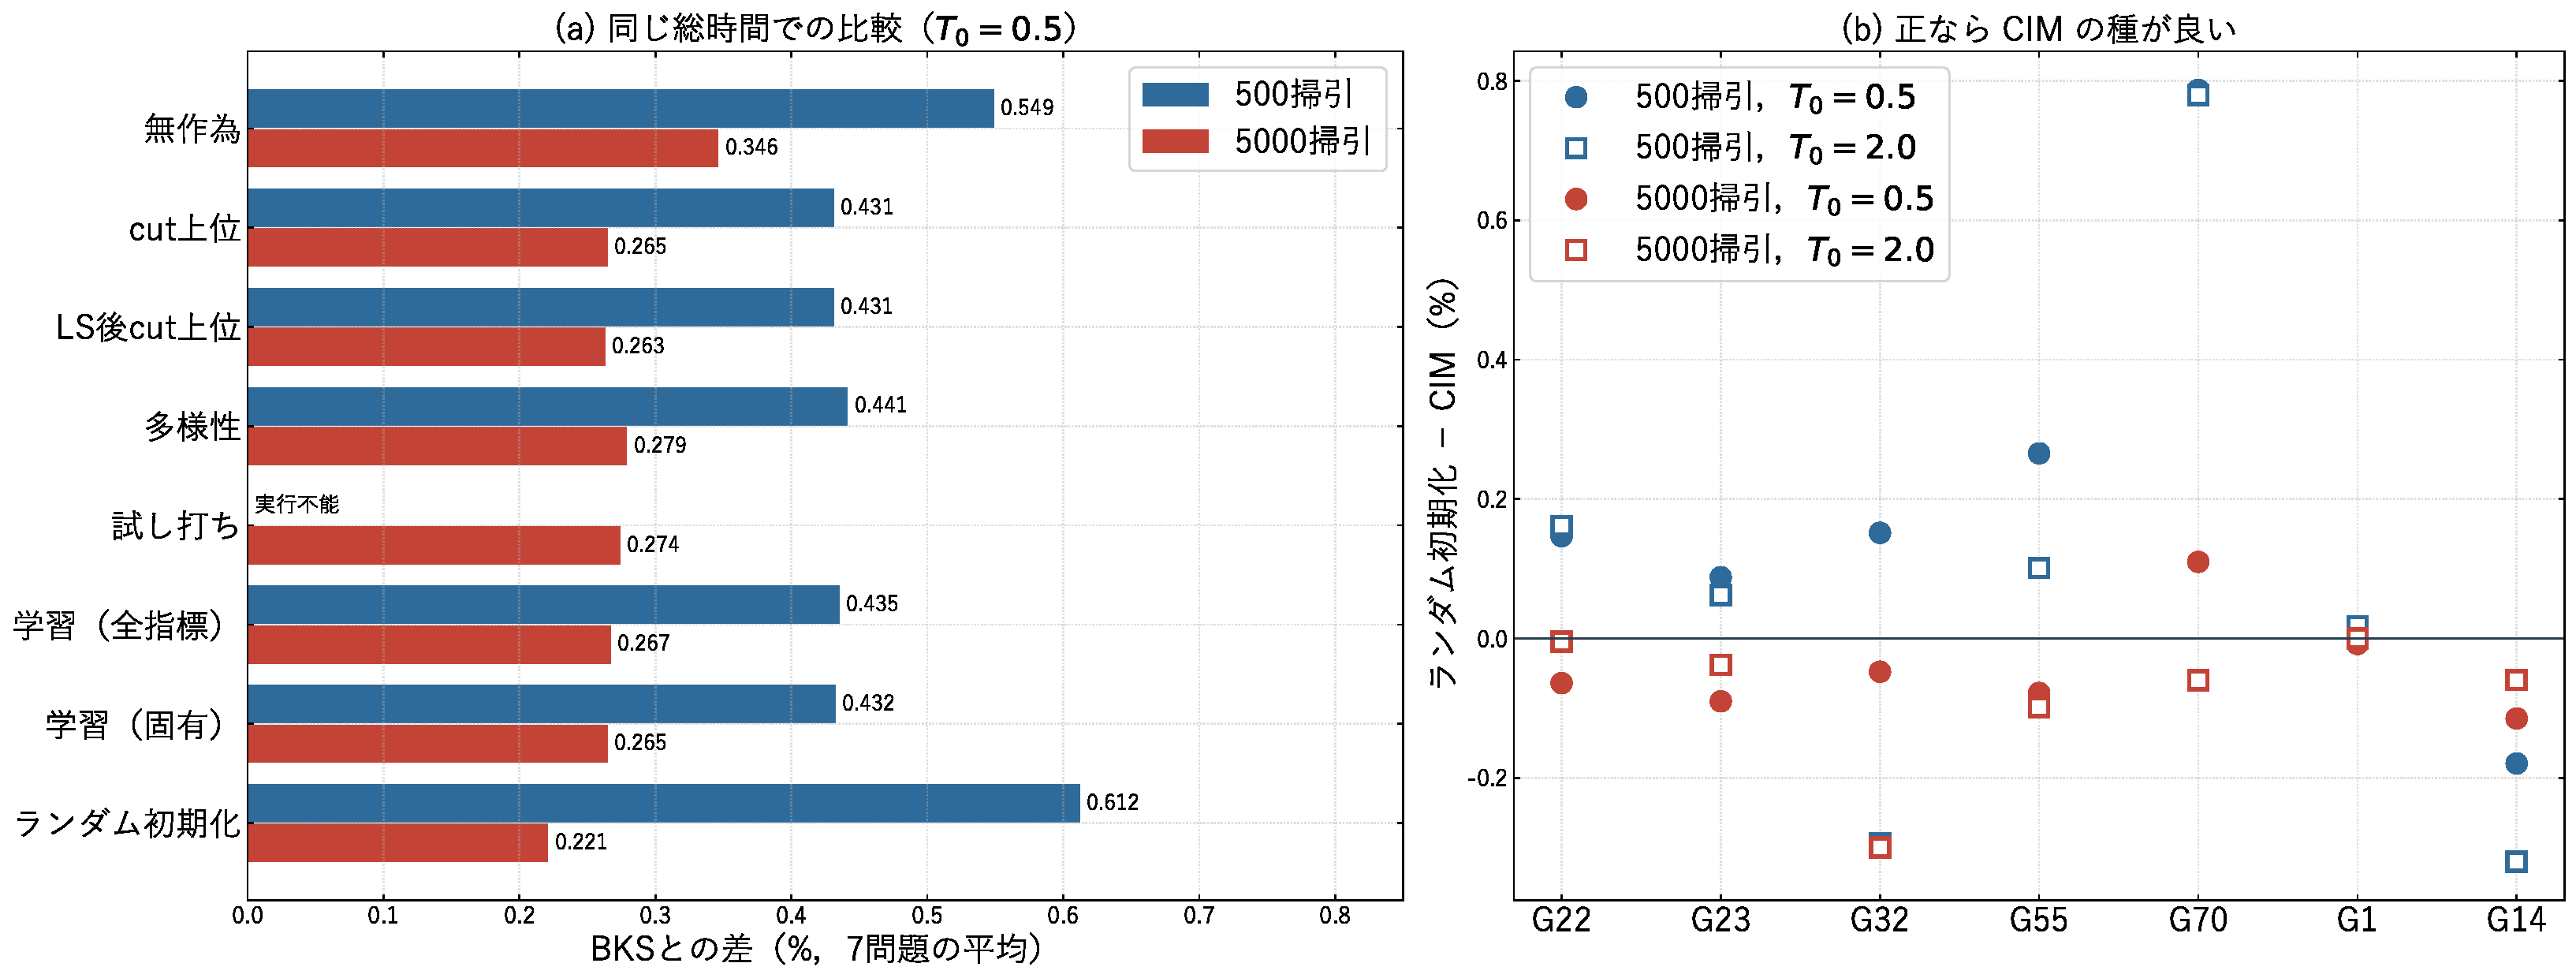
\includegraphics[width=\linewidth]{fig_selection.pdf}
\caption{(a) 主条件（$T_0=0.5$，$K=256$，$m=16$）での各方法の BKS との差．(b) 問題ごとの「ランダム初期化 $-$ LS 後 cut 上位」の BKS との差（正なら CIM の種が良い）．}\label{fig:selection}
\end{figure}

\paragraph{主条件では 3 つの判定がいずれも成り立たなかった.} 学習（全指標）は基準に対して 1 勝 6 敗（片側 $p=0.95$），試し打ちは 0 勝 7 敗（$p=1.00$）であり，基準はランダム初期化に対して 1 勝 6 敗（$p=0.92$）だった（表\ref{tab:selection}，図\ref{fig:selection}）．

\paragraph{カット値を超える選別は役に立たない.} 候補を無作為に選ぶより，カット値で選ぶほうがはるかに良い（主条件で BKS との差 0.346\% から 0.265\%）．しかし，カット値・LS 後のカット値を超える選別が基準を上回った幅は，8 条件のいずれでも，費用を 0 にした場合を含めて最大 0.003\% だった．費用を課すと，学習や試し打ちはむしろ悪くなった．試し打ちは 500 掃引では費用（50 掃引 × 2 回 × 候補数）が SA の予算全体を超え，実行できなかった．$m=4$ では LS の費用で SA が 1 本減るため，LS をしない「cut 上位」のほうが基準より良かった（$T_0=2.0$・5000 掃引で 0.375\% 対 0.394\%）．固有ベクトル指標が強く効く G22 の主条件でも，学習（固有ベクトル指標）の最良値の期待値は基準と変わらなかった（13349.3 対 13349.4）．

\paragraph{CIM の種の利点は予算が短いときに限られる.} CIM の種とランダム初期化の優劣は，後段の予算で逆転した（図\ref{fig:selection}(b)）．500 掃引では，CIM の種（基準）が 7 問題中 6 問題で良かった（$T_0=0.5$ で平均 0.431\% 対 0.612\%，片側 $p=0.039$，Holm 補正なしの副条件）．特に G70 では差が 0.79\% に達した．5000 掃引では逆に，ランダム初期化が 6 問題で良かった（0.263\% 対 0.221\%）．どちらの予算でも例外は 1 問題ずつだった（500 掃引では G14，5000 掃引では G70）．5000 掃引のランダム初期化は CIM の時間も SA に回すので，1 問題あたり 112〜171 本の SA を実行でき，16 本の CIM の種より最良値が伸びた．

\section{メメティックアルゴリズムと CIM の生成条件}\label{sec:ga}

\subsection{タブー探索の不具合と，CIM 初期集団の再評価}

メメティックアルゴリズム（GA）\cite{wu2012}は，交叉で作った子をタブー探索（TS）で磨き，距離と品質で集団を更新する．以前の実験では，G70 で CIM の解だけで作った初期集団の GA が 300 世代の間まったく改善せず，G55 では CIM 初期集団がランダムな初期集団より悪かった．原因を調べたところ，TS の実装が，利得が最大の非タブーの手が複数あるときに常に番号最小の頂点を選んでいた．疎なグラフの局所最適解には利得 0 の手が多数残るので，TS は同じ数頂点を往復し続け，局所最適解から動けなかった．Wu と Hao\cite{wu2012}にならい，同点の手を等確率に選び，摂動の強さを 150 にした．

同点を等確率に選ぶと，全頂点を走査しながら同点のたびに乱数を引くので，TS が遅くなった（40000 反復で G55 で 2.6 倍，G70 で 6.2 倍）．そこで，非タブーの頂点を利得の値ごとの配列（バケット）で管理し，最大利得のバケットから乱数 1 回で選ぶようにした．タブーの頂点はバケットから外してリストで管理し，aspiration はリストだけを調べる．選ぶ規則は全走査と同じであり，毎反復の状態を全走査の結果と照合する検査で食い違いがないことを確かめた．走査版に比べ，40000 反復で G22 で 2.8 倍，G55 で 31 倍，G70 で 87 倍速くなった．

修正後の TS で，以前と同じ seed・同じ初期集団（各問題 16 回，300 世代）の実験をやり直した（図\ref{fig:ga}）．G55 と G70 では結論が逆になった．300 世代後の BKS との差は，G55 で CIM 初期集団 $56.2\pm3.8$ に対しランダム $63.1\pm2.9$，G70 で $72.4\pm3.0$ に対し $92.2\pm3.6$（平均 $\pm$ 標準誤差）であり，CIM 初期集団のほうが良い．以前の「CIM 初期集団は GA の役に立たない」という結果は，TS の不具合によるものだった．G22 ではどちらも BKS との差 0.9 で差がなかった．この比較は同じ世代数での比較であり，CIM の生成時間は含めていない．生成時間を含めた比較は次の小節で行う．

\begin{figure}[t]
\centering
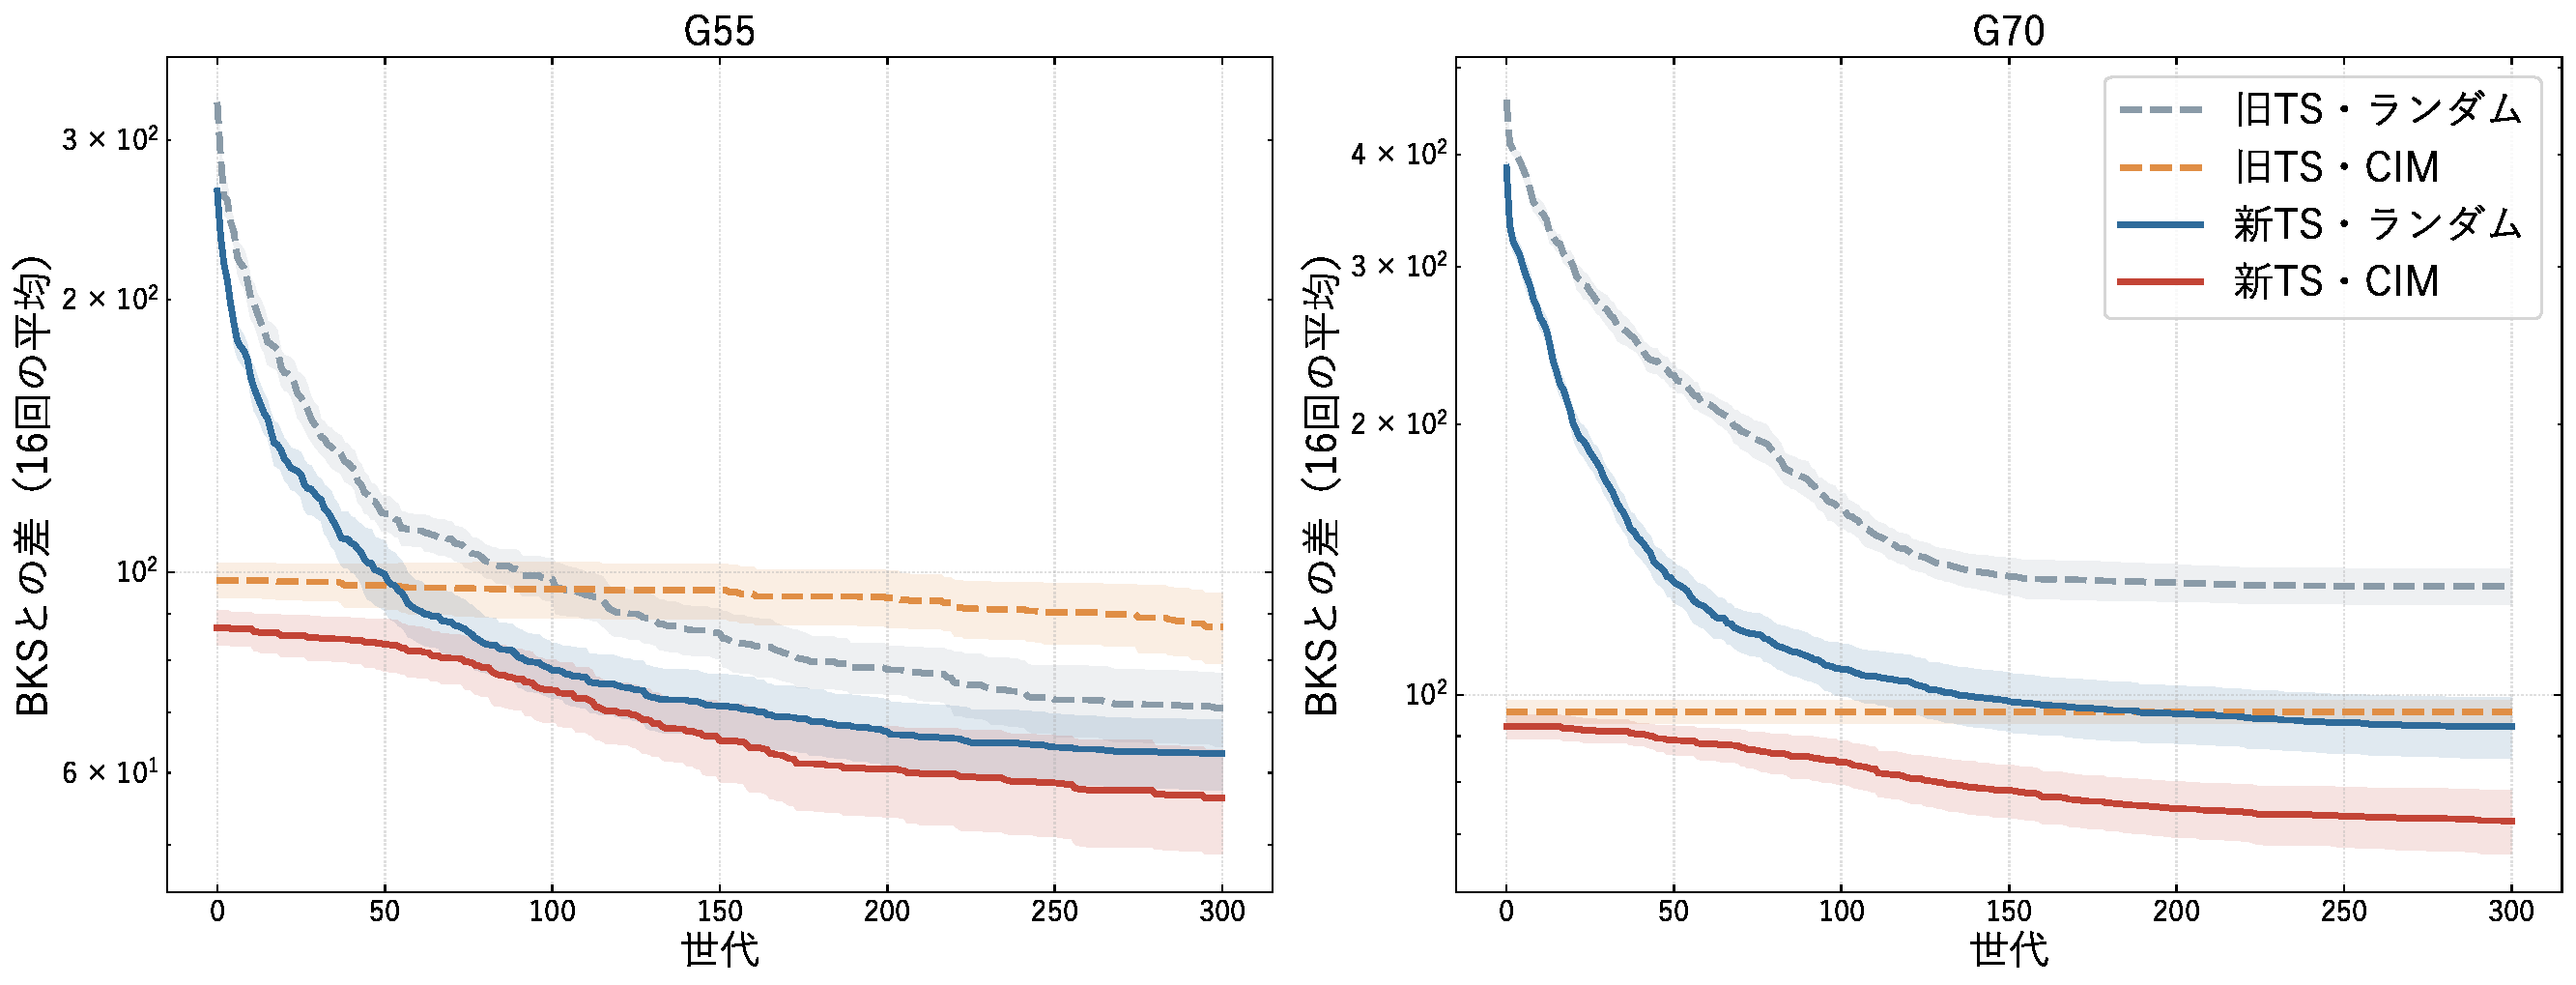
\includegraphics[width=\linewidth]{fig_ga.pdf}
\caption{GA の最良値の推移（BKS との差，16 回の平均と 95\% 区間）．破線は修正前の TS，実線は修正後の TS．同じ seed・同じ初期集団で比べた．}\label{fig:ga}
\end{figure}

\subsection{CIM の生成時間を含めた比較}\label{sec:ga_equal_time}

SA では，CIM の生成時間を後段に回すと，長い予算でランダムな初期解が勝った（\ref{sec:selection} 節）．GA でも同じことが起こるか，また，GA は交叉で解を組み合わせるので，SA では役に立たなかった多様な初期集団が効くかを調べた．条件と判定は実行前に文書に固定した．

問題は G22，G55，G70 で，GA のパラメータと CIM のラウンド数（G22・G70 は 4800，G55 は 9600）は前の小節と同じにした．GA と CIM はともに新しい seed で各問題 16 回実行した．各回で CIM の解を $K=4p$ 個（$p$ は集団サイズ）作り，初期集団を次の 4 通りで作った．\textbf{ランダム}は GA 既定の初期集団である．\textbf{CIM（選別なし）}は $K$ 個のうち seed 順に先頭の $p$ 個を使い，CIM の時間は $p$ 本分だけ課す．\textbf{CIM＋カット値}はカット値の上位 $p$ 個，\textbf{CIM＋カット値＋ハミング距離}はカット値の上位 $2p$ 個から互いに離れた $p$ 個を貪欲に選び，どちらも CIM の時間を $K$ 本分課す．どの条件も，初期集団に TS をかけてから世代を進める．

時間は，ほかの計算との重なりの影響を受けにくい 1 スレッドの CPU 時間で数えた．CIM 1 本の時間は GA の 1 世代の 32 倍（G22），124 倍（G55），147 倍（G70）だった．評価時刻は「CIM＋カット値が CIM の時間を払って 300 世代進む時刻」（40〜54 秒）とし，各回のその時刻までの最良値を比べた．CIM の時間の倍率 $c$ を 1（主条件）と，物理的な CIM で生成が速い場合を想定した 0.1，0 で変えた．判定は 2 つで，問題ごとに片側検定を行い，3 問題で Holm の補正をかけた．V4a：CIM（選別なし）がランダムより良い（Mann--Whitney の U 検定）．V4b：CIM＋カット値＋ハミング距離が CIM＋カット値より良い（同じ CIM の候補と GA の seed で対応があるので Wilcoxon の符号順位検定）．

\begin{table}[t]
\centering
\caption{CIM の生成時間を含めた GA の比較．評価時刻での BKS との差（\%，16 回の平均）．$c$ は CIM の時間に掛けた倍率．}\label{tab:ga_equal_time}
\small
\begin{tabular}{lccccc}
\toprule
問題 & $c$ & ランダム & CIM（選別なし） & CIM＋カット値 & CIM＋カット値＋距離 \\
\midrule
G22 & 1 & 0.014 & 0.006 & 0.007 & 0.007 \\
G55 & 1 & 0.502 & \textbf{0.316} & 0.441 & 0.572 \\
G55 & 0 & 0.502 & 0.312 & \textbf{0.284} & 0.323 \\
G70 & 1 & 0.861 & \textbf{0.609} & 0.684 & 0.880 \\
G70 & 0 & 0.861 & 0.589 & \textbf{0.556} & 0.754 \\
\bottomrule
\end{tabular}
\end{table}

\begin{figure}[t]
\centering
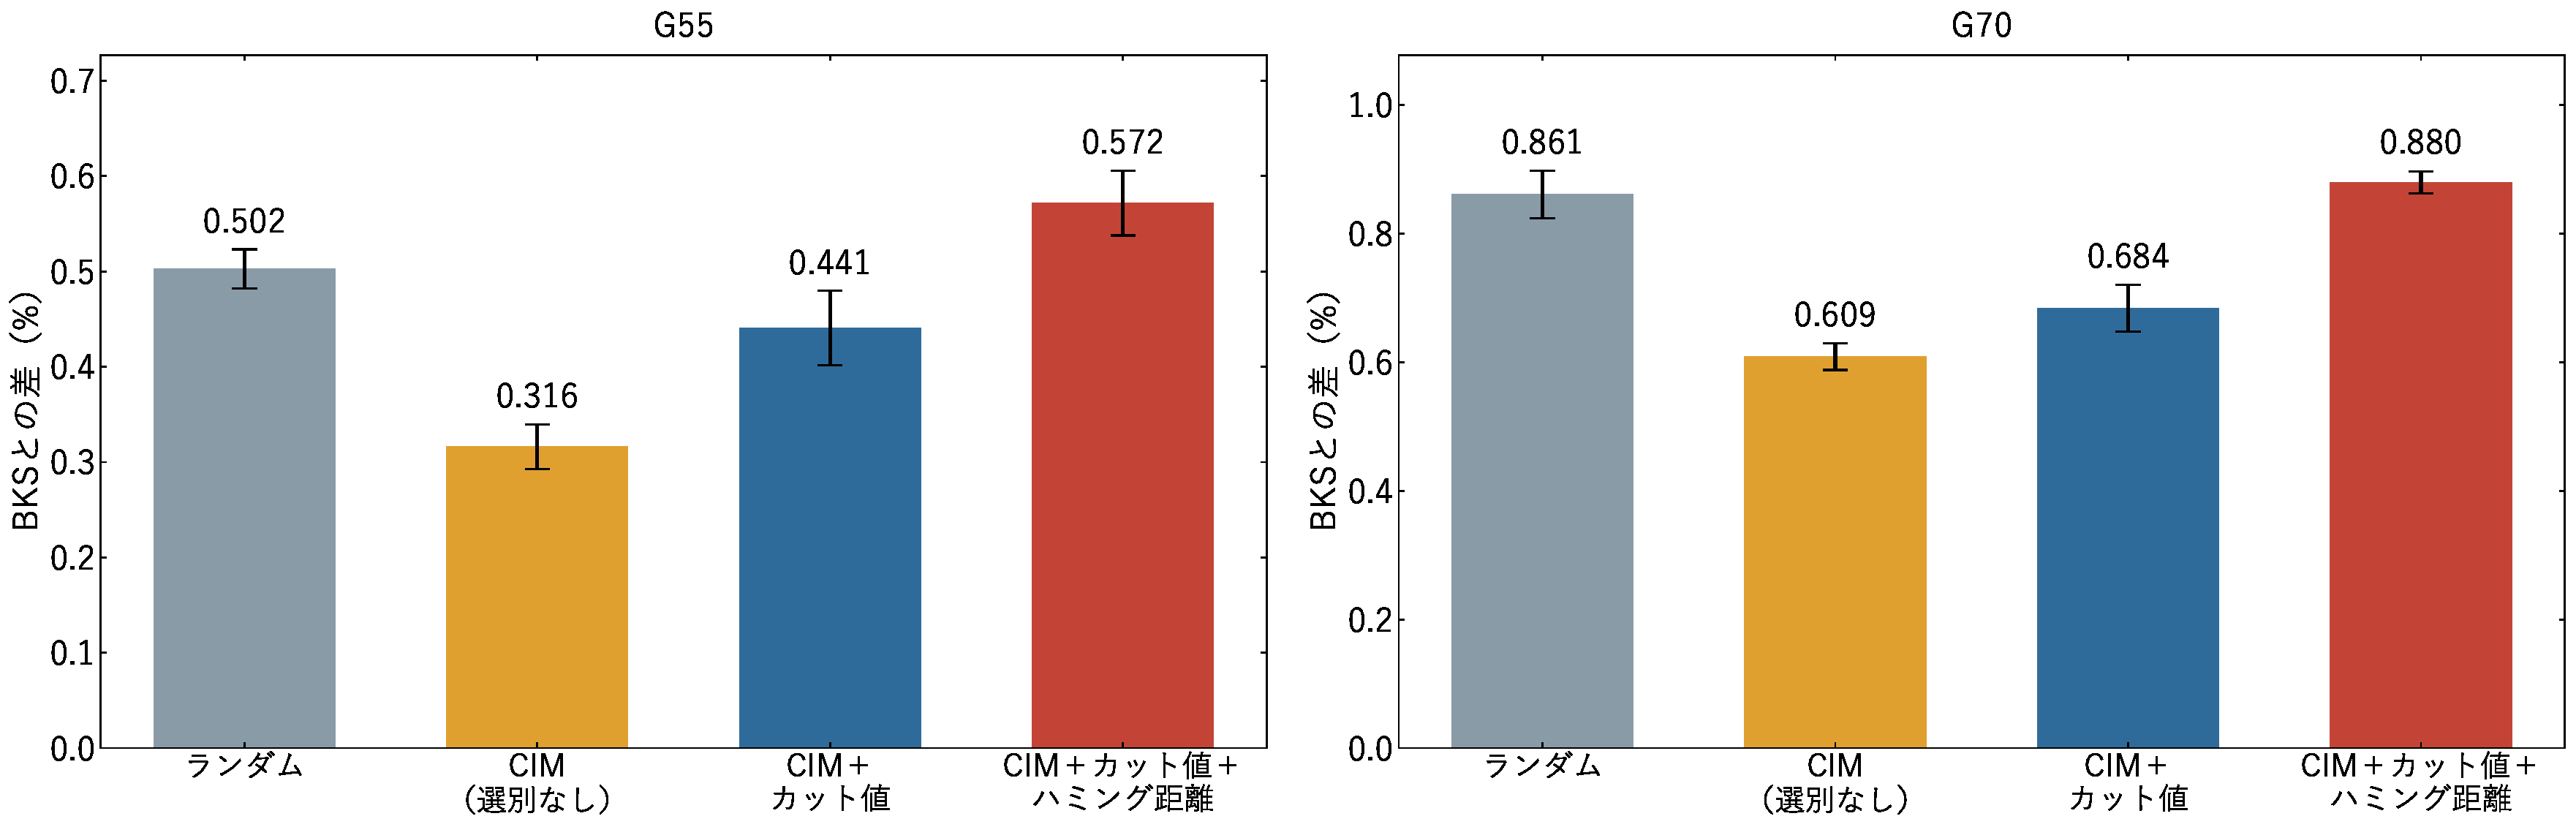
\includegraphics[width=\linewidth]{fig_ga_equal_time.pdf}
\caption{CIM の生成時間を含めた GA の比較（主条件 $c=1$）．評価時刻での BKS との差（16 回の平均と標準誤差）．}\label{fig:ga_equal_time}
\end{figure}

\paragraph{CIM の初期集団は生成時間を含めても良い（V4a 成立）.} G55 と G70 では，CIM（選別なし）がランダムより良かった（表\ref{tab:ga_equal_time}，図\ref{fig:ga_equal_time}．Holm 補正後 $p=2.2\times10^{-5}$，$1.5\times10^{-5}$）．G22 では全条件が BKS から 1〜2 しか離れず，差は出なかった（$p=0.55$）．実行前には，CIM の時間がランダムの数百〜千世代分に当たるので $c=1$ では成り立たないと予想していたが，この予想は外れた．時間と最良値の推移を見ると，ランダムな初期集団の GA は早い段階で伸びが止まる．CIM の初期集団の GA は，CIM の時間（G55 で約 10 秒，G70 で約 13 秒）を払った後，短時間でランダムを追い越し，その後も差が開いた．SA の長い予算と結果が逆になったのは，ランダムな初期解からの SA は本数を増やせば伸びるのに対し，GA の集団は一度停滞すると世代を重ねても抜け出しにくいためと考えられる．

\paragraph{多様な初期集団は役に立たない（V4b 不成立）.} ハミング距離で選んだ集団は，カット値だけで選んだ集団より悪かった（対応のある 16 回で G55 は 3 勝 13 敗，G70 は 1 勝 13 敗，Holm 補正後 $p=1.0$）．$c=0.1$，0 でも同じ向きだった．事後の診断では，各個体の最も近い相手との距離の平均は，G55 でカット値 0.235・選別なし 0.276・ハミング距離 0.320，G70 で 0.217・0.257・0.281 であり，$c=0$ での成績の順（カット値，選別なし，ハミング距離）と一致した．ハミング距離で選んだ集団は，選別なしより平均カット値が高いのに成績が悪い．この GA の交叉は親の共通部分を引き継ぐので，互いに近い個体の組がない集団では引き継げる部分が少ないためと考えられる（事後の解釈）．

\paragraph{時間の見積もりへの感度.} CIM 1 本の時間を 3 回の測定の最小値から中央値に変えた場合と，GA の 1 世代の時間を長い実行の傾きから求めた場合でも，V4a と V4b の判定は変わらなかった．ただし CIM＋カット値は，CIM の時間を中央値にすると評価時刻までに CIM の生成が終わらず，ランダムより悪くなった（G55 で 0.635\% 対 0.502\%）．評価時刻をこの条件に合わせて決めたため，この条件は時間の見積もりに最も敏感である．$c=1$ で CIM＋カット値が選別なしに負けたのも，$K=4p$ 本の CIM の時間を払うためであり，$c=0$ では逆にカット値で選ぶほうが良い．

\subsection{CIM の生成条件と固有ベクトルの系統}

G22 で，候補がどちらの固有ベクトルの系統に入るかを CIM の生成条件で変えられるかを調べた．事前登録の R1 と同じ設定（600 ラウンド，SA 開始温度 2.0・5000 掃引）を基準に，ポンプの立ち上げの速さ（ラウンド数と掛けた最終のポンプ強度は揃えた）と真空雑音の大きさを変え，各条件で新しい seed の候補 256 個に SA を 4 回ずつかけた（表\ref{tab:lineage}）．

\begin{table}[t]
\centering
\caption{G22 で CIM の生成条件を変えたときの候補（各 256 個）．$E>0$ は $u_1$ の系統に入った候補の割合．差は基準との差と 95\% 区間（独立 2 標本の正規近似）．}\label{tab:lineage}
\small
\begin{tabular}{lrcccc}
\toprule
条件 & ラウンド & 平均カット値 & $E>0$ の割合（基準との差） & SA 後の平均（基準との差） & $\rho(E, r)$ \\
\midrule
基準 & 600 & 13238.2 & 0.68 & 13331.0 & 0.44 \\
ポンプ 0.5 倍速 & 1200 & 13245.3 & $+0.06$ [$-0.02$, $0.13$] & $-1.0$ [$-3.5$, $1.5$] & 0.47 \\
ポンプ 2 倍速 & 300 & 13214.1 & $-0.11$ [$-0.20$, $-0.03$] & $-2.2$ [$-4.7$, $0.3$] & 0.45 \\
雑音 0.5 倍 & 600 & 13238.0 & $+0.01$ [$-0.07$, $0.09$] & $-0.1$ [$-2.7$, $2.5$] & 0.48 \\
雑音 2 倍 & 600 & 13237.4 & $-0.00$ [$-0.09$, $0.08$] & $+0.2$ [$-2.4$, $2.7$] & 0.45 \\
雑音 4 倍 & 600 & 13237.8 & $-0.01$ [$-0.09$, $0.07$] & $+0.3$ [$-2.3$, $2.8$] & 0.44 \\
\bottomrule
\end{tabular}
\end{table}

ポンプを速く立ち上げると，$u_1$ の系統に入る候補の割合が下がった（$-0.11$）．線形増幅の段階が短くなり，最大固有値のモードが他のモードに差をつける時間が減るためと考えられる．雑音の大きさは 0.5〜4 倍の範囲で影響しなかった．SA 後の平均は条件によって有意には変わらなかった．一方，$E$ と残差の相関はすべての条件で 0.44〜0.48 であり，G22 で $E$ が効くことは，新しい seed による 6 回の測定でも変わらなかった．系統の割合はポンプの速さで多少動かせるが，その効果は小さく，候補の選別に代わる手段にはならない．

\section{考察}\label{sec:discussion}

\subsection{種の価値の差はいつ現れるか}

同じカット値の候補の価値の差（C1）は，CIM の出力が多様なすべての問題で，種の近くを探す SA（$T_0=0.5$）では予算によらず成り立った．一方，開始温度が高い SA や長い予算では差が消えた．事前登録の実行で測った SA の出力と種の距離は，差が残った G22 で頂点の 26\%，差が消えた G55・G70 で 43〜44\% だった．全反転を同一視した無作為な 2 状態の距離の期待値は約 50\% なので，差が消えた条件では SA は種をほとんど忘れている．種の価値は，後段の探索が種の情報をどれだけ保つかで決まる量であり，候補だけの性質ではない．

小規模問題の全列挙では，価値は最適解までの距離（経路長）でほぼ決まり，障壁は弱かった．大規模問題でも，SA が種の近くを探す条件では「最適解への近さ」が効いていると考えるのが自然である．ただし，大規模問題では最適解が分からないので，この解釈は直接は確かめられない．

\subsection{固有ベクトル指標はなぜ一部の問題で効くか}

$E$ は G22 で事前登録どおりに再現し，G1 でも同じ大きさで成り立ったが，G23 や小規模問題の $\pm1$ 重みのグラフでは効かなかった．CIM の増幅の初期には $A$ の最小固有値側の固有ベクトルが最も速く成長し，ポンプを速く立ち上げて線形増幅の段階を短くすると，$u_1$ の系統に入る候補の割合が下がった（\ref{sec:ga} 節）．したがって $E$ は，候補が増幅の初期にどのモードに引き込まれたかの痕跡である．小規模問題で $a_1$ が最適解までの距離と相関したことから，$u_1$ の系統に入ることは，問題によっては最適解に近い領域に入ることを意味する．どの問題でそうなるかは，最適解と $u_1$ の符号パターンの重なりに依存するはずだが，本論文ではこれを予測する方法は見つけていない．

局所的な指標の向きが小規模問題と G-set で逆になったことも，指標の意味が問題の構造に依存することを示している．重み 1 のランダムグラフでは利得 $-2$〜$0$ の頂点が多いことが「動ける余地」として正に効き，小規模問題では「未完成の局所構造」として負に効いた可能性があるが，これは事後的な解釈である．問題をまたいで同じ向きに効いたのは試し打ちだけだった．試し打ちは後段の探索そのものの縮小版なので，問題の構造によらず効くのは自然である．

\subsection{なぜ選別は役に立たないか}

C1 と C2 が成り立つ問題でも，同じ総時間で比べると，カット値を超える選別の効果はほとんどなかった．理由は 3 つ考えられる．

第一に，カット値で説明できない価値の差は，カット値による差より小さい．無作為な選び方とカット値による選び方の差（主条件で BKS との差の平均 0.08\%）に比べ，カット値を超える選別で動かせた差（最大 0.003\%）は一桁以上小さかった．

第二に，評価量は $m$ 本の SA の\textbf{最良値}であり，価値（期待値）の差がそのまま最良値の差にはならない．カット値の上位の候補はすでに価値の高い群に入っていて，その中での順位の入れ替えは最良値をほとんど変えない．

第三に，選別の費用がかかる．LS と局所的な指標は SA に比べて十分安いが，試し打ちは短い予算では SA の予算全体より高くつく．固有ベクトルの計算は問題ごとに 1 回で済むが，それでも小さな $m$ では SA の本数を削る．

\subsection{CIM の種はいつ役に立つか}

CIM の種とランダム初期化の優劣は，後段の予算で逆転した．後段の予算が短いと，SA はランダムな初期解から良い解まで進めず，CIM の出力を出発点にできることの利点が大きい（G70 の 500 掃引では BKS との差で 0.79\% の改善）．後段の予算が長いと，SA はランダムな初期解からでも同程度の解に達し，CIM の生成時間を SA の本数に回したほうが最良値が伸びる．メメティックアルゴリズムでは，同じ世代数で比べると CIM の初期集団が G55・G70 で良かった（\ref{sec:ga} 節）．GA の後段は SA より強い探索だが，世代数が限られる場合には CIM の初期集団の品質が効くと考えられる．ただし，この比較は CIM の生成時間を含めていない．

実用上の示唆は次のとおりである．CIM を後段の探索の初期解生成に使うなら，(1) 候補はカット値（LS 後のカット値）で選べば十分であり，それ以上の選別に時間を使う価値は小さい．(2) CIM の生成時間を後段に回した場合との比較を必ず行うべきであり，後段の予算が長い設定では CIM を使わないほうが良いことがある．

\subsection{限界}

\begin{itemize}
  \item 小規模問題では，CIM がほぼ常に最適解を出すので，増幅の途中で止めた CIM の出力を候補とした．大規模問題の CIM の出力と性質が同じとは限らない．
  \item SA は途中の最良状態（初期解を含む）を返すので，開始温度が高く予算が短いとラベルが初期カット値と一致する．この条件は判定不能とし，判定不能の基準は結果を見てから改めた（\ref{sec:prereg}，\ref{sec:gset} 節）．
  \item 時間はすべて 1 台の計算機（24 スレッド）での実測であり，CIM は物理的な装置ではなく数値シミュレーションである．物理的な CIM では生成時間がはるかに短い可能性があり，その場合はランダム初期化との比較の結論が変わりうる．
  \item 平面グラフの G15・G39 では CIM の出力が 1〜5 状態に集まり，評価から除いた．CIM のパラメータ（結合の強さ以外）は G22 で調整した値であり，問題ごとに調整すれば多様性が増す可能性がある．
  \item G77 は計算時間の都合で除いた．比較は 7 問題で行い，問題を単位にした検定の検出力は低い．
  \item BKS は以前の研究で用いた既知の最良値の表に従った．値の出典によって BKS との差の絶対値は変わりうるが，同じ問題の中での方法の比較には影響しない．
\end{itemize}

\subsection{結論}

同じカット値の CIM 解は，後段の SA で同じ価値を持たない．この差は，SA が種の情報を保つ設定で，CIM の出力が多様なすべての問題で再現した．差の一部は，CIM の増幅の初期にどの固有ベクトルの系統に入ったかや，短い SA の試し打ちで予測できたが，効く指標は問題によって違った．そして，CIM の生成を含めた同じ総時間で比べると，カット値を超える選別は到達品質をほとんど改善しなかった．CIM の種が役に立つかどうかは，選別よりも，後段の探索にどれだけの予算を使うかで決まる．


\begin{thebibliography}{99}\small

\bibitem{wang2013} Z. Wang, A. Marandi, K. Wen, R. L. Byer, Y. Yamamoto, ``Coherent Ising machine based on degenerate optical parametric oscillators,'' \textit{Physical Review A}, 88, 063853, 2013.

\bibitem{inagaki2016} T. Inagaki \textit{et al.}, ``A coherent Ising machine for 2000-node optimization problems,'' \textit{Science}, 354(6312), 603--606, 2016.

\bibitem{mcmahon2016} P. L. McMahon \textit{et al.}, ``A fully programmable 100-spin coherent Ising machine with all-to-all connections,'' \textit{Science}, 354(6312), 614--617, 2016.

\bibitem{inoue2022} Inoue, Yoshida, ``Traveling-wave model of coherent Ising machine based on fiber loop with pulse-pumped phase-sensitive amplifier,'' \textit{Optics Communications}, 522, 128642, 2022.

\bibitem{haribara2015} Y. Haribara, S. Utsunomiya, Y. Yamamoto, ``A coherent Ising machine for MAX-CUT problems: performance evaluation against semidefinite programming relaxation and simulated annealing,'' arXiv:1501.07030, 2015.

\bibitem{leleu2019} T. Leleu, Y. Yamamoto, P. L. McMahon, K. Aihara, ``Destabilization of local minima in analog spin systems by correction of amplitude heterogeneity,'' \textit{Physical Review Letters}, 122, 040607, 2019.

\bibitem{goto2019} H. Goto, K. Tatsumura, A. R. Dixon, ``Combinatorial optimization by simulating adiabatic bifurcations in nonlinear Hamiltonian systems,'' \textit{Science Advances}, 5(4), eaav2372, 2019.

\bibitem{kirkpatrick1983} S. Kirkpatrick, C. D. Gelatt, M. P. Vecchi, ``Optimization by simulated annealing,'' \textit{Science}, 220(4598), 671--680, 1983.

\bibitem{goemans1995} M. X. Goemans, D. P. Williamson, ``Improved approximation algorithms for maximum cut and satisfiability problems using semidefinite programming,'' \textit{Journal of the ACM}, 42(6), 1115--1145, 1995.

\bibitem{helmberg2000} C. Helmberg, F. Rendl, ``A spectral bundle method for semidefinite programming,'' \textit{SIAM Journal on Optimization}, 10(3), 673--696, 2000.

\bibitem{wu2012} Q. Wu, J.-K. Hao, ``A memetic approach for the max-cut problem,'' in \textit{Parallel Problem Solving from Nature -- PPSN XII}, LNCS 7492, 297--306, 2012.

\bibitem{benlic2013} U. Benlic, J.-K. Hao, ``Breakout local search for the max-cut problem,'' \textit{Engineering Applications of Artificial Intelligence}, 26(3), 1162--1173, 2013.

\bibitem{ma2017} F. Ma, J.-K. Hao, ``A multiple search operator heuristic for the max-k-cut problem,'' \textit{Annals of Operations Research}, 248, 365--403, 2017（arXiv:1510.09156）.

\bibitem{dunning2018} I. Dunning, S. Gupta, J. Silberholz, ``What works best when? A systematic evaluation of heuristics for Max-Cut and QUBO,'' \textit{INFORMS Journal on Computing}, 30(3), 608--624, 2018.

\bibitem{ochoa2008} G. Ochoa, M. Tomassini, S. V\'{e}rel, C. Darabos, ``A study of NK landscapes' basins and local optima networks,'' in \textit{Proceedings of GECCO 2008}, 555--562, 2008.

\bibitem{barrett2020} T. D. Barrett, W. R. Clements, J. N. Foerster, A. I. Lvovsky, ``Exploratory combinatorial optimization with reinforcement learning,'' in \textit{Proceedings of AAAI 2020}, 3243--3250, 2020.

\bibitem{karnin2013} Z. Karnin, T. Koren, O. Somekh, ``Almost optimal exploration in multi-armed bandits,'' in \textit{Proceedings of ICML 2013}, 1238--1246, 2013.

\bibitem{jamieson2016} K. Jamieson, A. Talwalkar, ``Non-stochastic best arm identification and hyperparameter optimization,'' in \textit{Proceedings of AISTATS 2016}, 240--248, 2016.

\bibitem{trevisan2012} L. Trevisan, ``Max cut and the smallest eigenvalue,'' \textit{SIAM Journal on Computing}, 41(6), 1769--1786, 2012.

\bibitem{cosm2025} ``Performance report of heuristic algorithm that cracked the largest Gset Ising problems (G81 cut=14060),'' arXiv:2505.18508, 2025.

\end{thebibliography}

\appendix

\section{CIM のパラメータと時間}\label{app:timing}

表\ref{tab:timing}に，各問題の CIM の結合の強さと，\ref{sec:selection} 節の評価に使った時間を示す．G22・G55・G70 のパラメータは以前の研究で問題ごとに調整した値である（G55・G70 はポンプの立ち上げの速さも異なる）．ほかの問題は G22 の物理定数を使い，結合の強さだけを CIM 単体の平均カット値で選んだ．CIM と SA の時間は，ほかの計算がない状態で 24 スレッド（CIM は 512 本，SA は 512 本）で 2 回測った最小値を 1 本あたりに直した値である．LS・局所的な指標・内積は 1 スレッドで 512 候補を 3 回測った最小値の 1 候補あたりの値であり，評価ではこれを 24 で割った．固有ベクトルは問題ごとに 1 回だけ計算する．

\begin{table}[h]
\centering
\caption{CIM の結合の強さ $c$ と，各処理の時間．CIM は 2400 ラウンド，SA は $T_0=0.5$．}\label{tab:timing}
\small
\begin{tabular}{lrrrrrrrrr}
\toprule
 & & & CIM & \multicolumn{2}{c}{SA [ms]} & LS & 局所指標 & 内積 & 固有ベクトル \\
問題 & $n$ & $c$ & [ms] & 500 掃引 & 5000 掃引 & [$\mu$s] & [$\mu$s] & [$\mu$s] & [ms，1 回] \\
\midrule
G1 & 800 & $-0.01$ & 26.3 & 4.56 & 43.4 & 47 & 44 & 1.9 & 15 \\
G14 & 800 & $-0.05$ & 9.6 & 2.03 & 19.2 & 19 & 28 & 2.2 & 4 \\
G15 & 800 & $-0.03$ & 6.1 & 1.60 & 15.5 & 14 & 33 & 2.0 & 2 \\
G22 & 2000 & $-0.049$ & 20.5 & 4.78 & 45.0 & 42 & 96 & 4.9 & 15 \\
G23 & 2000 & $-0.05$ & 19.8 & 4.85 & 45.1 & 54 & 95 & 4.5 & 16 \\
G32 & 2000 & $-0.08$ & 10.1 & 2.74 & 27.0 & 21 & 69 & 6.5 & 11 \\
G39 & 2000 & $-0.03$ & 14.8 & 4.11 & 41.5 & 60 & 100 & 5.7 & 7 \\
G55 & 5000 & $-0.130$ & 39.8 & 9.83 & 100.2 & 111 & 352 & 16.5 & 31 \\
G70 & 10000 & $-0.153$ & 64.2 & 16.34 & 156.9 & 230 & 680 & 34.8 & 62 \\
\bottomrule
\end{tabular}
\end{table}

\section{タブー探索の高速化}\label{app:tabu}

同点を等確率に選ぶ TS では，毎反復で全頂点の利得を走査し，最大利得の非タブーの頂点から 1 つを等確率に選ぶ．重みが整数なら利得は $[-D, D]$（$D$ は重み付き次数の最大値）の整数なので，非タブーの頂点を利得の値ごとの配列（バケット）に入れ，各頂点の配列内の位置を記録しておけば，挿入と削除は定数時間でできる．最大利得のバケットは上から探し，そこから乱数 1 回で選ぶ．反転した頂点の隣接頂点だけ利得が変わるので，1 反復の費用は次数に比例する．タブーの頂点はバケットから外してリストで管理し，毎反復でリストを調べて，期間が終わった頂点をバケットに戻す．aspiration（タブーでも，反転すれば最良値を更新する手は許す）の候補も，このリストを調べるときに同時に探せばよい．最良状態のコピーは，最良状態から離れる手の直前にだけ取る．検査モードでは毎反復，バケットの内容と全走査で求めた候補の集合が一致することを確かめ，G22 と $\pm1$ 重みの疎・密なグラフで食い違いがないことを確認した．

\section{結果を見た後に変えた点}\label{app:changes}

事前登録と実行前の計画から，結果を見た後に変えた点をまとめる．いずれも変更前の出力をリポジトリに残した．
\begin{enumerate}
  \item 事前登録：SA が種を一度も超えずラベルが初期カット値と一致する条件を判定不能とした（\ref{sec:prereg} 節）．主予算の判定には影響しない．
  \item 事前登録：探索段階の「二峰性」の記述を，判定基準を当てはめた結果に合わせて訂正した（\ref{sec:prereg} 節）．
  \item G-set の検証：計算時間の都合で，結果を見る前に G77 を除いた．
  \item G-set の検証：判定不能の基準を「SA が種を一度でも超えた候補が 5\% 未満」に改めた（\ref{sec:gset} 節）．3 条件が判定不能になった．
  \item 選別の評価：費用を処理ごとに測り直し，方法ごとに使う処理だけを課した．ランダム初期化の SA を 4096 本に増やして非復元抽出にした．時間をほかの計算がない状態で測り直した（\ref{sec:selection} 節）．主条件の判定はどの版でも同じだった．
\end{enumerate}

\section{再現の手順}\label{app:repro}

すべてのスクリプトはリポジトリのルートから実行する．主な対応は次のとおりである．
\begin{itemize}\raggedright
  \item 事前登録：\texttt{docs/20261018/prereg\_eigen\_v1.md}，\texttt{scripts/benchmarks/seed\_value\_pilot.py}，\texttt{prereg\_eigen\_analysis.py}．
  \item 小規模問題：\texttt{docs/20261018/step2\_dev\_decisions.md}，\texttt{small\_landscape.py}，\texttt{small\_seed\_study.py}，\texttt{small\_seed\_analysis.py}．
  \item G-set の検証：\texttt{docs/20261018/step3\_plan.md}，\texttt{gset\_seed\_analysis.py}，\texttt{gset\_seed\_judge.py}．
  \item 選別の評価：\texttt{docs/20261018/step4\_plan.md}，\texttt{random\_init\_sa.py}，\texttt{selection\_costs.py}，\texttt{pipeline\_timing.py}，\texttt{selection\_eval.py}．
  \item GA と CIM の生成条件：\texttt{modules/GA.py}，\texttt{modules/tabu\_bucket.py}，\texttt{cim\_condition\_lineage.py}．
  \item 図：\texttt{scripts/plotting/paper\_figures.py}．
\end{itemize}
結果は \texttt{results/2026-10-18/} と \texttt{results/2026-10-19/} の下に，実験の種類と版ごとに保存した．

\end{document}
